\documentclass[twoside]{book}

% Packages required by doxygen
\usepackage{calc}
\usepackage{doxygen}
\usepackage{graphicx}
\usepackage[utf8]{inputenc}
\usepackage{makeidx}
\usepackage{multicol}
\usepackage{multirow}
\usepackage{textcomp}
\usepackage[table]{xcolor}

% NLS support packages
\usepackage[T2A]{fontenc}
\usepackage[ukrainian]{babel}

% Font selection
\usepackage[T1]{fontenc}
\usepackage{mathptmx}
\usepackage[scaled=.90]{helvet}
\usepackage{courier}
\usepackage{amssymb}
\usepackage{sectsty}
\renewcommand{\familydefault}{\sfdefault}
\allsectionsfont{%
  \fontseries{bc}\selectfont%
  \color{darkgray}%
}
\renewcommand{\DoxyLabelFont}{%
  \fontseries{bc}\selectfont%
  \color{darkgray}%
}

% Page & text layout
\usepackage{geometry}
\geometry{%
  a4paper,%
  top=2.5cm,%
  bottom=2.5cm,%
  left=2.5cm,%
  right=2.5cm%
}
\tolerance=750
\hfuzz=15pt
\hbadness=750
\setlength{\emergencystretch}{15pt}
\setlength{\parindent}{0cm}
\setlength{\parskip}{0.2cm}
\makeatletter
\renewcommand{\paragraph}{%
  \@startsection{paragraph}{4}{0ex}{-1.0ex}{1.0ex}{%
    \normalfont\normalsize\bfseries\SS@parafont%
  }%
}
\renewcommand{\subparagraph}{%
  \@startsection{subparagraph}{5}{0ex}{-1.0ex}{1.0ex}{%
    \normalfont\normalsize\bfseries\SS@subparafont%
  }%
}
\makeatother

% Headers & footers
\usepackage{fancyhdr}
\pagestyle{fancyplain}
\fancyhead[LE]{\fancyplain{}{\bfseries\thepage}}
\fancyhead[CE]{\fancyplain{}{}}
\fancyhead[RE]{\fancyplain{}{\bfseries\leftmark}}
\fancyhead[LO]{\fancyplain{}{\bfseries\rightmark}}
\fancyhead[CO]{\fancyplain{}{}}
\fancyhead[RO]{\fancyplain{}{\bfseries\thepage}}
\fancyfoot[LE]{\fancyplain{}{}}
\fancyfoot[CE]{\fancyplain{}{}}
\fancyfoot[RE]{\fancyplain{}{\bfseries\scriptsize Документація до Recognitor створена Вівторок, 22 липня 2014 23\-:58\-:27 системою Doxygen }}
\fancyfoot[LO]{\fancyplain{}{\bfseries\scriptsize Документація до Recognitor створена Вівторок, 22 липня 2014 23\-:58\-:27 системою Doxygen }}
\fancyfoot[CO]{\fancyplain{}{}}
\fancyfoot[RO]{\fancyplain{}{}}
\renewcommand{\footrulewidth}{0.4pt}
\renewcommand{\chaptermark}[1]{%
  \markboth{#1}{}%
}
\renewcommand{\sectionmark}[1]{%
  \markright{\thesection\ #1}%
}

% Indices & bibliography
\usepackage{natbib}
\usepackage[titles]{tocloft}
\setcounter{tocdepth}{3}
\setcounter{secnumdepth}{5}
\makeindex

% Hyperlinks (required, but should be loaded last)
\usepackage{ifpdf}
\ifpdf
  \usepackage[pdftex,pagebackref=true]{hyperref}
\else
  \usepackage[ps2pdf,pagebackref=true]{hyperref}
\fi
\hypersetup{%
  colorlinks=true,%
  linkcolor=blue,%
  citecolor=blue,%
  unicode%
}

% Custom commands
\newcommand{\clearemptydoublepage}{%
  \newpage{\pagestyle{empty}\cleardoublepage}%
}


%===== C O N T E N T S =====

\begin{document}

% Titlepage & ToC
\hypersetup{pageanchor=false}
\pagenumbering{roman}
\begin{titlepage}
\vspace*{7cm}
\begin{center}%
{\Large Recognitor }\\
\vspace*{1cm}
{\large Створено системою Doxygen 1.8.6}\\
\vspace*{0.5cm}
{\small Вівторок, 22 липня 2014 23:58:27}\\
\end{center}
\end{titlepage}
\clearemptydoublepage
\tableofcontents
\clearemptydoublepage
\pagenumbering{arabic}
\hypersetup{pageanchor=true}

%--- Begin generated contents ---
\chapter{Ієрархічний покажчик класів}
\section{Ієрархія класів}
Список успадкувань впорядковано наближено до алфавіту\begin{DoxyCompactList}
\item \contentsline{section}{Admin\-Screen}{\pageref{classAdminScreen}}{}
\item \contentsline{section}{A\-R\-G\-S}{\pageref{structARGS}}{}
\item \contentsline{section}{Camera\-Capture}{\pageref{classCameraCapture}}{}
\item \contentsline{section}{Ex\-User\-Screen}{\pageref{classExUserScreen}}{}
\item \contentsline{section}{Goods\-Mgmt\-Screen}{\pageref{classGoodsMgmtScreen}}{}
\item \contentsline{section}{Main\-Window}{\pageref{classMainWindow}}{}
\item \contentsline{section}{Packet}{\pageref{classPacket}}{}
\item \contentsline{section}{Ui\-\_\-\-Admin\-Screen}{\pageref{classUi__AdminScreen}}{}
\begin{DoxyCompactList}
\item \contentsline{section}{Ui\-:\-:Admin\-Screen}{\pageref{classUi_1_1AdminScreen}}{}
\end{DoxyCompactList}
\item \contentsline{section}{Ui\-\_\-\-Ex\-User\-Screen}{\pageref{classUi__ExUserScreen}}{}
\begin{DoxyCompactList}
\item \contentsline{section}{Ui\-:\-:Ex\-User\-Screen}{\pageref{classUi_1_1ExUserScreen}}{}
\end{DoxyCompactList}
\item \contentsline{section}{Ui\-\_\-\-Goods\-Mgmt\-Screen}{\pageref{classUi__GoodsMgmtScreen}}{}
\begin{DoxyCompactList}
\item \contentsline{section}{Ui\-:\-:Goods\-Mgmt\-Screen}{\pageref{classUi_1_1GoodsMgmtScreen}}{}
\end{DoxyCompactList}
\item \contentsline{section}{Ui\-\_\-\-Main\-Window}{\pageref{classUi__MainWindow}}{}
\begin{DoxyCompactList}
\item \contentsline{section}{Ui\-:\-:Main\-Window}{\pageref{classUi_1_1MainWindow}}{}
\end{DoxyCompactList}
\item \contentsline{section}{Ui\-\_\-\-User\-Screen}{\pageref{classUi__UserScreen}}{}
\begin{DoxyCompactList}
\item \contentsline{section}{Ui\-:\-:User\-Screen}{\pageref{classUi_1_1UserScreen}}{}
\end{DoxyCompactList}
\item \contentsline{section}{User\-Screen}{\pageref{classUserScreen}}{}
\item \contentsline{section}{Window\-Manager}{\pageref{classWindowManager}}{}
\end{DoxyCompactList}

\chapter{Алфавітний покажчик класів}
\section{Класи}
Класи, структури, об'єднання та інтерфейси з коротким описом.\begin{DoxyCompactList}
\item\contentsline{section}{\hyperlink{classAdminScreen}{Admin\-Screen} \\*Administrator window class }{\pageref{classAdminScreen}}{}
\item\contentsline{section}{\hyperlink{classUi_1_1AdminScreen}{Ui\-::\-Admin\-Screen} }{\pageref{classUi_1_1AdminScreen}}{}
\item\contentsline{section}{\hyperlink{structARGS}{A\-R\-G\-S} \\*The arguments for the capturing thread function }{\pageref{structARGS}}{}
\item\contentsline{section}{\hyperlink{classCameraCapture}{Camera\-Capture} \\*A class for capturing frames from the camera }{\pageref{classCameraCapture}}{}
\item\contentsline{section}{\hyperlink{classExUserScreen}{Ex\-User\-Screen} \\*Extended User window class }{\pageref{classExUserScreen}}{}
\item\contentsline{section}{\hyperlink{classUi_1_1ExUserScreen}{Ui\-::\-Ex\-User\-Screen} }{\pageref{classUi_1_1ExUserScreen}}{}
\item\contentsline{section}{\hyperlink{classUi_1_1GoodsMgmtScreen}{Ui\-::\-Goods\-Mgmt\-Screen} }{\pageref{classUi_1_1GoodsMgmtScreen}}{}
\item\contentsline{section}{\hyperlink{classGoodsMgmtScreen}{Goods\-Mgmt\-Screen} \\*Goods Management window class }{\pageref{classGoodsMgmtScreen}}{}
\item\contentsline{section}{\hyperlink{classImShowable}{Im\-Showable} }{\pageref{classImShowable}}{}
\item\contentsline{section}{\hyperlink{classUi_1_1MainWindow}{Ui\-::\-Main\-Window} }{\pageref{classUi_1_1MainWindow}}{}
\item\contentsline{section}{\hyperlink{classMainWindow}{Main\-Window} \\*Main window class }{\pageref{classMainWindow}}{}
\item\contentsline{section}{\hyperlink{classPacket}{Packet} \\*A class for Client-\/\-Server communication }{\pageref{classPacket}}{}
\item\contentsline{section}{\hyperlink{classResponsive}{Responsive} }{\pageref{classResponsive}}{}
\item\contentsline{section}{\hyperlink{classUi__AdminScreen}{Ui\-\_\-\-Admin\-Screen} }{\pageref{classUi__AdminScreen}}{}
\item\contentsline{section}{\hyperlink{classUi__ExUserScreen}{Ui\-\_\-\-Ex\-User\-Screen} }{\pageref{classUi__ExUserScreen}}{}
\item\contentsline{section}{\hyperlink{classUi__GoodsMgmtScreen}{Ui\-\_\-\-Goods\-Mgmt\-Screen} }{\pageref{classUi__GoodsMgmtScreen}}{}
\item\contentsline{section}{\hyperlink{classUi__MainWindow}{Ui\-\_\-\-Main\-Window} }{\pageref{classUi__MainWindow}}{}
\item\contentsline{section}{\hyperlink{classUi__UserScreen}{Ui\-\_\-\-User\-Screen} }{\pageref{classUi__UserScreen}}{}
\item\contentsline{section}{\hyperlink{classUserScreen}{User\-Screen} \\*User window class }{\pageref{classUserScreen}}{}
\item\contentsline{section}{\hyperlink{classUi_1_1UserScreen}{Ui\-::\-User\-Screen} }{\pageref{classUi_1_1UserScreen}}{}
\item\contentsline{section}{\hyperlink{classWindowManager}{Window\-Manager} \\*A class for switching between windows of the application }{\pageref{classWindowManager}}{}
\end{DoxyCompactList}

\chapter{Покажчик файлв}
\section{Файли}
Повний список документованих файлів.\begin{DoxyCompactList}
\item\contentsline{section}{Recognitor-\/build-\/desktop-\/\-Qt\-\_\-4\-\_\-8\-\_\-3\-\_\-in\-\_\-\-P\-A\-T\-H\-\_\-\-\_\-\-System\-\_\-\-\_\-\-Release/{\bfseries ui\-\_\-adminscreen.\-h} }{\pageref{ui__adminscreen_8h}}{}
\item\contentsline{section}{Recognitor-\/build-\/desktop-\/\-Qt\-\_\-4\-\_\-8\-\_\-3\-\_\-in\-\_\-\-P\-A\-T\-H\-\_\-\-\_\-\-System\-\_\-\-\_\-\-Release/{\bfseries ui\-\_\-exuserscreen.\-h} }{\pageref{ui__exuserscreen_8h}}{}
\item\contentsline{section}{Recognitor-\/build-\/desktop-\/\-Qt\-\_\-4\-\_\-8\-\_\-3\-\_\-in\-\_\-\-P\-A\-T\-H\-\_\-\-\_\-\-System\-\_\-\-\_\-\-Release/{\bfseries ui\-\_\-goodsmgmtscreen.\-h} }{\pageref{ui__goodsmgmtscreen_8h}}{}
\item\contentsline{section}{Recognitor-\/build-\/desktop-\/\-Qt\-\_\-4\-\_\-8\-\_\-3\-\_\-in\-\_\-\-P\-A\-T\-H\-\_\-\-\_\-\-System\-\_\-\-\_\-\-Release/{\bfseries ui\-\_\-mainwindow.\-h} }{\pageref{ui__mainwindow_8h}}{}
\item\contentsline{section}{Recognitor-\/build-\/desktop-\/\-Qt\-\_\-4\-\_\-8\-\_\-3\-\_\-in\-\_\-\-P\-A\-T\-H\-\_\-\-\_\-\-System\-\_\-\-\_\-\-Release/{\bfseries ui\-\_\-userscreen.\-h} }{\pageref{ui__userscreen_8h}}{}
\item\contentsline{section}{Recognitor/\hyperlink{adminscreen_8cpp}{adminscreen.\-cpp} \\*Administration window implementation }{\pageref{adminscreen_8cpp}}{}
\item\contentsline{section}{Recognitor/\hyperlink{adminscreen_8h}{adminscreen.\-h} \\*Administration window header }{\pageref{adminscreen_8h}}{}
\item\contentsline{section}{Recognitor/\hyperlink{auth_8cpp}{auth.\-cpp} \\*Authentication implementation }{\pageref{auth_8cpp}}{}
\item\contentsline{section}{Recognitor/\hyperlink{auth_8h}{auth.\-h} \\*Authentication header }{\pageref{auth_8h}}{}
\item\contentsline{section}{Recognitor/\hyperlink{cameracapture_8cpp}{cameracapture.\-cpp} \\*Camera capturing class implementation }{\pageref{cameracapture_8cpp}}{}
\item\contentsline{section}{Recognitor/\hyperlink{cameracapture_8h}{cameracapture.\-h} \\*Camera capturing class header }{\pageref{cameracapture_8h}}{}
\item\contentsline{section}{Recognitor/\hyperlink{cvtoqt_8cpp}{cvtoqt.\-cpp} \\*Open\-C\-V-\/\-Qt conversion implementation }{\pageref{cvtoqt_8cpp}}{}
\item\contentsline{section}{Recognitor/\hyperlink{cvtoqt_8h}{cvtoqt.\-h} \\*Open\-C\-V-\/\-Qt conversion header }{\pageref{cvtoqt_8h}}{}
\item\contentsline{section}{Recognitor/\hyperlink{exuserscreen_8cpp}{exuserscreen.\-cpp} \\*Extended User window implementation }{\pageref{exuserscreen_8cpp}}{}
\item\contentsline{section}{Recognitor/\hyperlink{exuserscreen_8h}{exuserscreen.\-h} \\*Extended User window header }{\pageref{exuserscreen_8h}}{}
\item\contentsline{section}{Recognitor/\hyperlink{goodsmgmtscreen_8cpp}{goodsmgmtscreen.\-cpp} \\*Goods management window implementation }{\pageref{goodsmgmtscreen_8cpp}}{}
\item\contentsline{section}{Recognitor/\hyperlink{goodsmgmtscreen_8h}{goodsmgmtscreen.\-h} \\*Goods management window header }{\pageref{goodsmgmtscreen_8h}}{}
\item\contentsline{section}{Recognitor/{\bfseries imshowable.\-h} }{\pageref{imshowable_8h}}{}
\item\contentsline{section}{Recognitor/\hyperlink{main_8cpp}{main.\-cpp} \\*Main source file }{\pageref{main_8cpp}}{}
\item\contentsline{section}{Recognitor/\hyperlink{mainwindow_8cpp}{mainwindow.\-cpp} \\*Authorization window source }{\pageref{mainwindow_8cpp}}{}
\item\contentsline{section}{Recognitor/\hyperlink{mainwindow_8h}{mainwindow.\-h} \\*Authorization window header (auto generated) }{\pageref{mainwindow_8h}}{}
\item\contentsline{section}{Recognitor/\hyperlink{packet_8cpp}{packet.\-cpp} \\*\hyperlink{classPacket}{Packet} class implementation }{\pageref{packet_8cpp}}{}
\item\contentsline{section}{Recognitor/\hyperlink{packet_8h}{packet.\-h} \\*\hyperlink{classPacket}{Packet} class header }{\pageref{packet_8h}}{}
\item\contentsline{section}{Recognitor/{\bfseries responsive.\-h} }{\pageref{responsive_8h}}{}
\item\contentsline{section}{Recognitor/\hyperlink{userscreen_8cpp}{userscreen.\-cpp} \\*User window implementation }{\pageref{userscreen_8cpp}}{}
\item\contentsline{section}{Recognitor/\hyperlink{userscreen_8h}{userscreen.\-h} \\*User window header }{\pageref{userscreen_8h}}{}
\item\contentsline{section}{Recognitor/\hyperlink{windowmanager_8cpp}{windowmanager.\-cpp} \\*Window switcher class implementation }{\pageref{windowmanager_8cpp}}{}
\item\contentsline{section}{Recognitor/\hyperlink{windowmanager_8h}{windowmanager.\-h} \\*Window switcher class header }{\pageref{windowmanager_8h}}{}
\end{DoxyCompactList}

\chapter{Класи}
\hypertarget{classAdminScreen}{\section{Клас Admin\-Screen}
\label{classAdminScreen}\index{Admin\-Screen@{Admin\-Screen}}
}
\subsection*{Загальнодоступні елементи}
\begin{DoxyCompactItemize}
\item 
\hyperlink{classAdminScreen_afacdce9a29c025265097914529ff5619}{Admin\-Screen} (Q\-Widget $\ast$parent=0)
\begin{DoxyCompactList}\small\item\em \hyperlink{classAdminScreen}{Admin\-Screen} constructor. \end{DoxyCompactList}\item 
\hypertarget{classAdminScreen_afaf1ed51e4a07af841c11f0f354ad2ed}{\hyperlink{classAdminScreen_afaf1ed51e4a07af841c11f0f354ad2ed}{$\sim$\-Admin\-Screen} ()}\label{classAdminScreen_afaf1ed51e4a07af841c11f0f354ad2ed}

\begin{DoxyCompactList}\small\item\em \hyperlink{classAdminScreen}{Admin\-Screen} destructor. \end{DoxyCompactList}\end{DoxyCompactItemize}


\subsection{Конструктор(и)}
\hypertarget{classAdminScreen_afacdce9a29c025265097914529ff5619}{\index{Admin\-Screen@{Admin\-Screen}!Admin\-Screen@{Admin\-Screen}}
\index{Admin\-Screen@{Admin\-Screen}!AdminScreen@{Admin\-Screen}}
\subsubsection[{Admin\-Screen}]{\setlength{\rightskip}{0pt plus 5cm}Admin\-Screen\-::\-Admin\-Screen (
\begin{DoxyParamCaption}
\item[{Q\-Widget $\ast$}]{parent = {\ttfamily 0}}
\end{DoxyParamCaption}
)\hspace{0.3cm}{\ttfamily [explicit]}}}\label{classAdminScreen_afacdce9a29c025265097914529ff5619}


\hyperlink{classAdminScreen}{Admin\-Screen} constructor. 


\begin{DoxyParams}[1]{Аргументи}
\mbox{\tt in}  & {\em parent} & -\/ Window parent \\
\hline
\end{DoxyParams}


Документація цих класів була створена з файлів\-:\begin{DoxyCompactItemize}
\item 
Recognitor/\hyperlink{adminscreen_8h}{adminscreen.\-h}\item 
Recognitor/\hyperlink{adminscreen_8cpp}{adminscreen.\-cpp}\end{DoxyCompactItemize}

\hypertarget{classUi_1_1AdminScreen}{\section{Клас Ui\-:\-:Admin\-Screen}
\label{classUi_1_1AdminScreen}\index{Ui\-::\-Admin\-Screen@{Ui\-::\-Admin\-Screen}}
}
Схема успадкувань для Ui\-:\-:Admin\-Screen\begin{figure}[H]
\begin{center}
\leavevmode
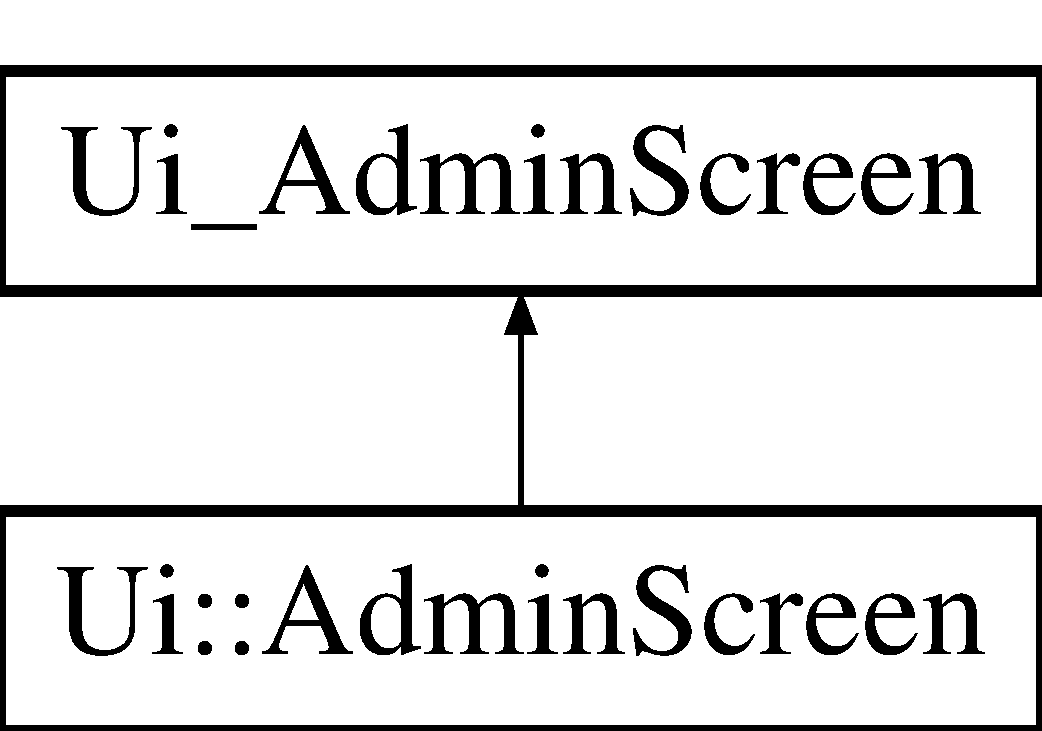
\includegraphics[height=2.000000cm]{classUi_1_1AdminScreen}
\end{center}
\end{figure}
\subsection*{Додаткові успадковані елементи}


Документація цього класу була створена з файлу\-:\begin{DoxyCompactItemize}
\item 
Recognitor/ui\-\_\-adminscreen.\-h\end{DoxyCompactItemize}

\hypertarget{structARGS}{\section{Структура A\-R\-G\-S}
\label{structARGS}\index{A\-R\-G\-S@{A\-R\-G\-S}}
}


The arguments for the capturing thread function.  




{\ttfamily \#include $<$cameracapture.\-h$>$}

\subsection*{Загальнодоступні атрибути}
\begin{DoxyCompactItemize}
\item 
\hypertarget{structARGS_af74ee694152c4be9de805a3fe7b709dc}{pthread\-\_\-t \hyperlink{structARGS_af74ee694152c4be9de805a3fe7b709dc}{pid}}\label{structARGS_af74ee694152c4be9de805a3fe7b709dc}

\begin{DoxyCompactList}\small\item\em Capturing thread handle. \end{DoxyCompactList}\item 
\hypertarget{structARGS_a6b299867eec1febb4d3ed313ac73f0d7}{cv\-::\-Video\-Capture $\ast$ \hyperlink{structARGS_a6b299867eec1febb4d3ed313ac73f0d7}{cap}}\label{structARGS_a6b299867eec1febb4d3ed313ac73f0d7}

\begin{DoxyCompactList}\small\item\em Video\-Capture object. \end{DoxyCompactList}\item 
\hypertarget{structARGS_a761da80183bdbfbf9a293c9ba1130d2c}{Q\-Widget $\ast$ \hyperlink{structARGS_a761da80183bdbfbf9a293c9ba1130d2c}{parent}}\label{structARGS_a761da80183bdbfbf9a293c9ba1130d2c}

\begin{DoxyCompactList}\small\item\em Parent object (caller) \end{DoxyCompactList}\end{DoxyCompactItemize}


\subsection{Детальний опис}
The arguments for the capturing thread function. 

\begin{DoxySeeAlso}{Див. також}
lf() 
\end{DoxySeeAlso}


Документація цієї структури була створена з файлу\-:\begin{DoxyCompactItemize}
\item 
Recognitor/\hyperlink{cameracapture_8h}{cameracapture.\-h}\end{DoxyCompactItemize}

\hypertarget{classCameraCapture}{\section{Клас Camera\-Capture}
\label{classCameraCapture}\index{Camera\-Capture@{Camera\-Capture}}
}


A class for capturing frames from the camera.  




{\ttfamily \#include $<$cameracapture.\-h$>$}

\subsection*{Загальнодоступні елементи}
\begin{DoxyCompactItemize}
\item 
\hyperlink{classCameraCapture_a110d7f3ede7cb2e2b24584a9700abd2f}{Camera\-Capture} (Q\-Widget $\ast$par)
\begin{DoxyCompactList}\small\item\em \hyperlink{classCameraCapture}{Camera\-Capture} constructor. \end{DoxyCompactList}\item 
\hypertarget{classCameraCapture_a1ab7b68c620d79769afb3920320250fe}{void \hyperlink{classCameraCapture_a1ab7b68c620d79769afb3920320250fe}{Start} ()}\label{classCameraCapture_a1ab7b68c620d79769afb3920320250fe}

\begin{DoxyCompactList}\small\item\em This function does initialization and starts the capturing thread. \end{DoxyCompactList}\item 
\hypertarget{classCameraCapture_ab29bec18aca2752893b0dcd6b1870cc9}{void \hyperlink{classCameraCapture_ab29bec18aca2752893b0dcd6b1870cc9}{End} ()}\label{classCameraCapture_ab29bec18aca2752893b0dcd6b1870cc9}

\begin{DoxyCompactList}\small\item\em This function cancels the capturing thread. \end{DoxyCompactList}\end{DoxyCompactItemize}
\subsection*{Приватні дані}
\begin{DoxyCompactItemize}
\item 
\hypertarget{classCameraCapture_aa288f3da7bc3cea5f568b64e75a65eaf}{cv\-::\-Video\-Capture $\ast$ {\bfseries cap}}\label{classCameraCapture_aa288f3da7bc3cea5f568b64e75a65eaf}

\item 
\hypertarget{classCameraCapture_ad0703a036cc45c2f8b74c873bca6b5db}{pthread\-\_\-t \hyperlink{classCameraCapture_ad0703a036cc45c2f8b74c873bca6b5db}{pid}}\label{classCameraCapture_ad0703a036cc45c2f8b74c873bca6b5db}

\begin{DoxyCompactList}\small\item\em Capturing thread handle. \end{DoxyCompactList}\item 
\hypertarget{classCameraCapture_a7ef70abf92c37be8a342dd8d728a6b03}{Q\-Widget $\ast$ \hyperlink{classCameraCapture_a7ef70abf92c37be8a342dd8d728a6b03}{parent}}\label{classCameraCapture_a7ef70abf92c37be8a342dd8d728a6b03}

\begin{DoxyCompactList}\small\item\em Parent for creating Q\-Message\-Box`es. \end{DoxyCompactList}\end{DoxyCompactItemize}


\subsection{Детальний опис}
A class for capturing frames from the camera. 

\subsection{Конструктор(и)}
\hypertarget{classCameraCapture_a110d7f3ede7cb2e2b24584a9700abd2f}{\index{Camera\-Capture@{Camera\-Capture}!Camera\-Capture@{Camera\-Capture}}
\index{Camera\-Capture@{Camera\-Capture}!CameraCapture@{Camera\-Capture}}
\subsubsection[{Camera\-Capture}]{\setlength{\rightskip}{0pt plus 5cm}Camera\-Capture\-::\-Camera\-Capture (
\begin{DoxyParamCaption}
\item[{Q\-Widget $\ast$}]{par}
\end{DoxyParamCaption}
)}}\label{classCameraCapture_a110d7f3ede7cb2e2b24584a9700abd2f}


\hyperlink{classCameraCapture}{Camera\-Capture} constructor. 


\begin{DoxyParams}[1]{Аргументи}
\mbox{\tt in}  & {\em par} & -\/ Parent for creating Q\-Message\-Box`es\\
\hline
\end{DoxyParams}
\begin{DoxyReturn}{Повертає}
Q\-Image Converted from cv\-::\-Mat 
\end{DoxyReturn}


Документація цих класів була створена з файлів\-:\begin{DoxyCompactItemize}
\item 
Recognitor/\hyperlink{cameracapture_8h}{cameracapture.\-h}\item 
Recognitor/\hyperlink{cameracapture_8cpp}{cameracapture.\-cpp}\end{DoxyCompactItemize}

\hypertarget{classExUserScreen}{\section{Клас Ex\-User\-Screen}
\label{classExUserScreen}\index{Ex\-User\-Screen@{Ex\-User\-Screen}}
}
\subsection*{Загальнодоступні елементи}
\begin{DoxyCompactItemize}
\item 
\hyperlink{classExUserScreen_a8642db4f09c4528daf7e22ce2dcc1b47}{Ex\-User\-Screen} (Q\-Widget $\ast$parent=0)
\begin{DoxyCompactList}\small\item\em \hyperlink{classExUserScreen}{Ex\-User\-Screen} constructor. \end{DoxyCompactList}\item 
\hypertarget{classExUserScreen_a61421cd56bb9b54501c4cb34d297891f}{\hyperlink{classExUserScreen_a61421cd56bb9b54501c4cb34d297891f}{$\sim$\-Ex\-User\-Screen} ()}\label{classExUserScreen_a61421cd56bb9b54501c4cb34d297891f}

\begin{DoxyCompactList}\small\item\em \hyperlink{classExUserScreen}{Ex\-User\-Screen} destructor. \end{DoxyCompactList}\end{DoxyCompactItemize}
\subsection*{Приватні слоти}
\begin{DoxyCompactItemize}
\item 
\hypertarget{classExUserScreen_a30a26ad349a33bac86a0848934c55655}{void \hyperlink{classExUserScreen_a30a26ad349a33bac86a0848934c55655}{on\-\_\-push\-Button\-\_\-2\-\_\-clicked} ()}\label{classExUserScreen_a30a26ad349a33bac86a0848934c55655}

\begin{DoxyCompactList}\small\item\em Exit button click handler. \end{DoxyCompactList}\item 
\hypertarget{classExUserScreen_a4c7d4f567fc5d87bf459c4fe9ae09411}{void \hyperlink{classExUserScreen_a4c7d4f567fc5d87bf459c4fe9ae09411}{on\-\_\-push\-Button\-\_\-clicked} ()}\label{classExUserScreen_a4c7d4f567fc5d87bf459c4fe9ae09411}

\begin{DoxyCompactList}\small\item\em Start button click handler. \end{DoxyCompactList}\item 
\hypertarget{classExUserScreen_ad5eeeac687e031eb0b722957b20191cf}{void \hyperlink{classExUserScreen_ad5eeeac687e031eb0b722957b20191cf}{on\-\_\-push\-Button\-\_\-3\-\_\-clicked} ()}\label{classExUserScreen_ad5eeeac687e031eb0b722957b20191cf}

\begin{DoxyCompactList}\small\item\em Manage Goods button click handler. \end{DoxyCompactList}\end{DoxyCompactItemize}
\subsection*{Приватні дані}
\begin{DoxyCompactItemize}
\item 
\hypertarget{classExUserScreen_abed6a95638d506058d3b1e6e69a42788}{\hyperlink{classUi_1_1ExUserScreen}{Ui\-::\-Ex\-User\-Screen} $\ast$ \hyperlink{classExUserScreen_abed6a95638d506058d3b1e6e69a42788}{ui}}\label{classExUserScreen_abed6a95638d506058d3b1e6e69a42788}

\begin{DoxyCompactList}\small\item\em User interface reference. \end{DoxyCompactList}\end{DoxyCompactItemize}


\subsection{Конструктор(и)}
\hypertarget{classExUserScreen_a8642db4f09c4528daf7e22ce2dcc1b47}{\index{Ex\-User\-Screen@{Ex\-User\-Screen}!Ex\-User\-Screen@{Ex\-User\-Screen}}
\index{Ex\-User\-Screen@{Ex\-User\-Screen}!ExUserScreen@{Ex\-User\-Screen}}
\subsubsection[{Ex\-User\-Screen}]{\setlength{\rightskip}{0pt plus 5cm}Ex\-User\-Screen\-::\-Ex\-User\-Screen (
\begin{DoxyParamCaption}
\item[{Q\-Widget $\ast$}]{parent = {\ttfamily 0}}
\end{DoxyParamCaption}
)\hspace{0.3cm}{\ttfamily [explicit]}}}\label{classExUserScreen_a8642db4f09c4528daf7e22ce2dcc1b47}


\hyperlink{classExUserScreen}{Ex\-User\-Screen} constructor. 


\begin{DoxyParams}[1]{Аргументи}
\mbox{\tt in}  & {\em parent} & -\/ Window parent \\
\hline
\end{DoxyParams}


Документація цих класів була створена з файлів\-:\begin{DoxyCompactItemize}
\item 
Recognitor/\hyperlink{exuserscreen_8h}{exuserscreen.\-h}\item 
Recognitor/\hyperlink{exuserscreen_8cpp}{exuserscreen.\-cpp}\end{DoxyCompactItemize}

\hypertarget{classUi_1_1ExUserScreen}{\section{Клас Ui\-:\-:Ex\-User\-Screen}
\label{classUi_1_1ExUserScreen}\index{Ui\-::\-Ex\-User\-Screen@{Ui\-::\-Ex\-User\-Screen}}
}
Схема успадкувань для Ui\-:\-:Ex\-User\-Screen\begin{figure}[H]
\begin{center}
\leavevmode
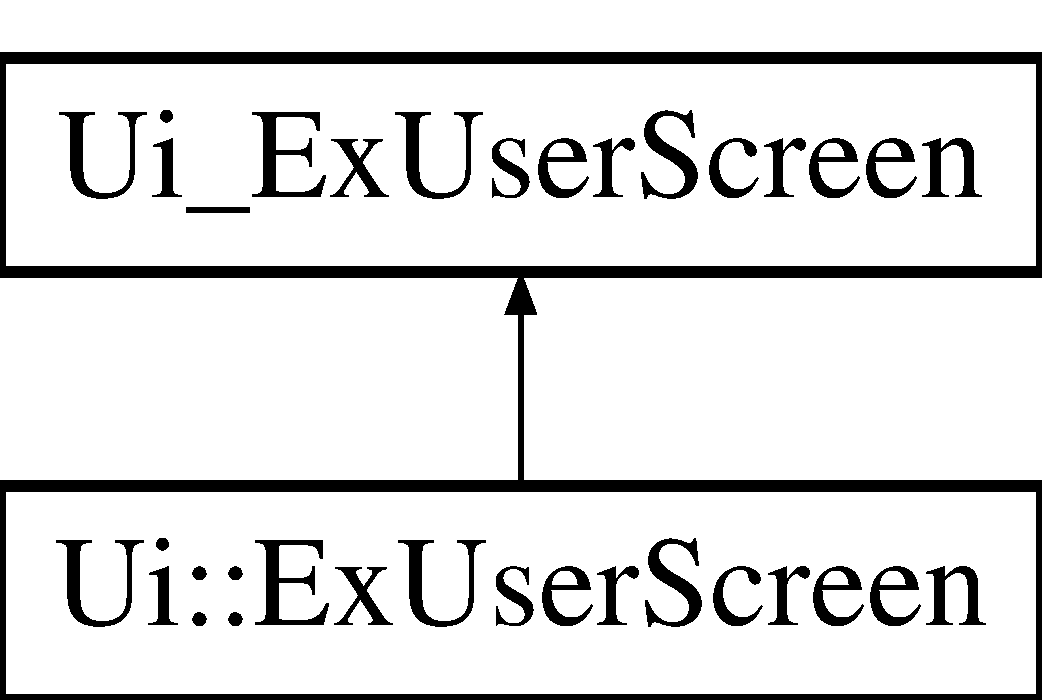
\includegraphics[height=2.000000cm]{classUi_1_1ExUserScreen}
\end{center}
\end{figure}
\subsection*{Додаткові успадковані елементи}


Документація цього класу була створена з файлу\-:\begin{DoxyCompactItemize}
\item 
Recognitor/ui\-\_\-exuserscreen.\-h\end{DoxyCompactItemize}

\hypertarget{classGoodsMgmtScreen}{\section{Клас Goods\-Mgmt\-Screen}
\label{classGoodsMgmtScreen}\index{Goods\-Mgmt\-Screen@{Goods\-Mgmt\-Screen}}
}
\subsection*{Загальнодоступні елементи}
\begin{DoxyCompactItemize}
\item 
\hyperlink{classGoodsMgmtScreen_a23df1d60103959e1b6fc32852aec9873}{Goods\-Mgmt\-Screen} (Q\-Widget $\ast$parent=0)
\begin{DoxyCompactList}\small\item\em \hyperlink{classGoodsMgmtScreen}{Goods\-Mgmt\-Screen} constructor. \end{DoxyCompactList}\item 
\hypertarget{classGoodsMgmtScreen_a0ab5666478d7b8fa00843aa127ce2a3b}{\hyperlink{classGoodsMgmtScreen_a0ab5666478d7b8fa00843aa127ce2a3b}{$\sim$\-Goods\-Mgmt\-Screen} ()}\label{classGoodsMgmtScreen_a0ab5666478d7b8fa00843aa127ce2a3b}

\begin{DoxyCompactList}\small\item\em \hyperlink{classGoodsMgmtScreen}{Goods\-Mgmt\-Screen} destructor. \end{DoxyCompactList}\end{DoxyCompactItemize}
\subsection*{Приватні слоти}
\begin{DoxyCompactItemize}
\item 
\hypertarget{classGoodsMgmtScreen_af6b7ddc269f16db33def62a0c088cd72}{void \hyperlink{classGoodsMgmtScreen_af6b7ddc269f16db33def62a0c088cd72}{on\-\_\-push\-Button\-\_\-clicked} ()}\label{classGoodsMgmtScreen_af6b7ddc269f16db33def62a0c088cd72}

\begin{DoxyCompactList}\small\item\em Add Item button click handler. \end{DoxyCompactList}\item 
\hypertarget{classGoodsMgmtScreen_ad7e09acd2978457ccba9ca4829218837}{void \hyperlink{classGoodsMgmtScreen_ad7e09acd2978457ccba9ca4829218837}{on\-\_\-push\-Button\-\_\-2\-\_\-clicked} ()}\label{classGoodsMgmtScreen_ad7e09acd2978457ccba9ca4829218837}

\begin{DoxyCompactList}\small\item\em Edit Item button click handler. \end{DoxyCompactList}\item 
\hypertarget{classGoodsMgmtScreen_a8ad921cd256c2847ae9505619ea05e31}{void \hyperlink{classGoodsMgmtScreen_a8ad921cd256c2847ae9505619ea05e31}{on\-\_\-push\-Button\-\_\-3\-\_\-clicked} ()}\label{classGoodsMgmtScreen_a8ad921cd256c2847ae9505619ea05e31}

\begin{DoxyCompactList}\small\item\em Remove Item button click handler. \end{DoxyCompactList}\item 
\hypertarget{classGoodsMgmtScreen_a28787cbd6ab01f8b874983658c27b39b}{void \hyperlink{classGoodsMgmtScreen_a28787cbd6ab01f8b874983658c27b39b}{on\-\_\-push\-Button\-\_\-4\-\_\-clicked} ()}\label{classGoodsMgmtScreen_a28787cbd6ab01f8b874983658c27b39b}

\begin{DoxyCompactList}\small\item\em Exit button click handler. \end{DoxyCompactList}\end{DoxyCompactItemize}
\subsection*{Приватні дані}
\begin{DoxyCompactItemize}
\item 
\hypertarget{classGoodsMgmtScreen_ac3a8443017075cfa943106952464f494}{\hyperlink{classUi_1_1GoodsMgmtScreen}{Ui\-::\-Goods\-Mgmt\-Screen} $\ast$ \hyperlink{classGoodsMgmtScreen_ac3a8443017075cfa943106952464f494}{ui}}\label{classGoodsMgmtScreen_ac3a8443017075cfa943106952464f494}

\begin{DoxyCompactList}\small\item\em User interface reference. \end{DoxyCompactList}\end{DoxyCompactItemize}


\subsection{Конструктор(и)}
\hypertarget{classGoodsMgmtScreen_a23df1d60103959e1b6fc32852aec9873}{\index{Goods\-Mgmt\-Screen@{Goods\-Mgmt\-Screen}!Goods\-Mgmt\-Screen@{Goods\-Mgmt\-Screen}}
\index{Goods\-Mgmt\-Screen@{Goods\-Mgmt\-Screen}!GoodsMgmtScreen@{Goods\-Mgmt\-Screen}}
\subsubsection[{Goods\-Mgmt\-Screen}]{\setlength{\rightskip}{0pt plus 5cm}Goods\-Mgmt\-Screen\-::\-Goods\-Mgmt\-Screen (
\begin{DoxyParamCaption}
\item[{Q\-Widget $\ast$}]{parent = {\ttfamily 0}}
\end{DoxyParamCaption}
)\hspace{0.3cm}{\ttfamily [explicit]}}}\label{classGoodsMgmtScreen_a23df1d60103959e1b6fc32852aec9873}


\hyperlink{classGoodsMgmtScreen}{Goods\-Mgmt\-Screen} constructor. 


\begin{DoxyParams}[1]{Аргументи}
\mbox{\tt in}  & {\em parent} & -\/ Window parent \\
\hline
\end{DoxyParams}


Документація цих класів була створена з файлів\-:\begin{DoxyCompactItemize}
\item 
Recognitor/\hyperlink{goodsmgmtscreen_8h}{goodsmgmtscreen.\-h}\item 
Recognitor/\hyperlink{goodsmgmtscreen_8cpp}{goodsmgmtscreen.\-cpp}\end{DoxyCompactItemize}

\hypertarget{classUi_1_1GoodsMgmtScreen}{\section{Клас Ui\-:\-:Goods\-Mgmt\-Screen}
\label{classUi_1_1GoodsMgmtScreen}\index{Ui\-::\-Goods\-Mgmt\-Screen@{Ui\-::\-Goods\-Mgmt\-Screen}}
}
Схема успадкувань для Ui\-:\-:Goods\-Mgmt\-Screen\begin{figure}[H]
\begin{center}
\leavevmode
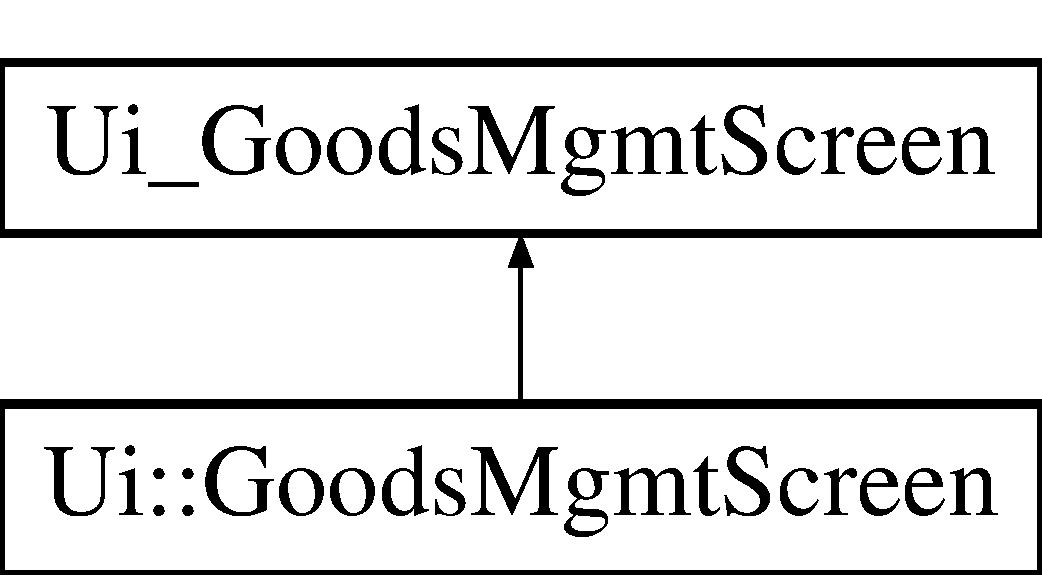
\includegraphics[height=2.000000cm]{classUi_1_1GoodsMgmtScreen}
\end{center}
\end{figure}
\subsection*{Додаткові успадковані елементи}


Документація цього класу була створена з файлу\-:\begin{DoxyCompactItemize}
\item 
Recognitor/ui\-\_\-goodsmgmtscreen.\-h\end{DoxyCompactItemize}

\hypertarget{classkeyEnterReceiver}{\section{Клас key\-Enter\-Receiver}
\label{classkeyEnterReceiver}\index{key\-Enter\-Receiver@{key\-Enter\-Receiver}}
}
Схема успадкувань для key\-Enter\-Receiver\begin{figure}[H]
\begin{center}
\leavevmode
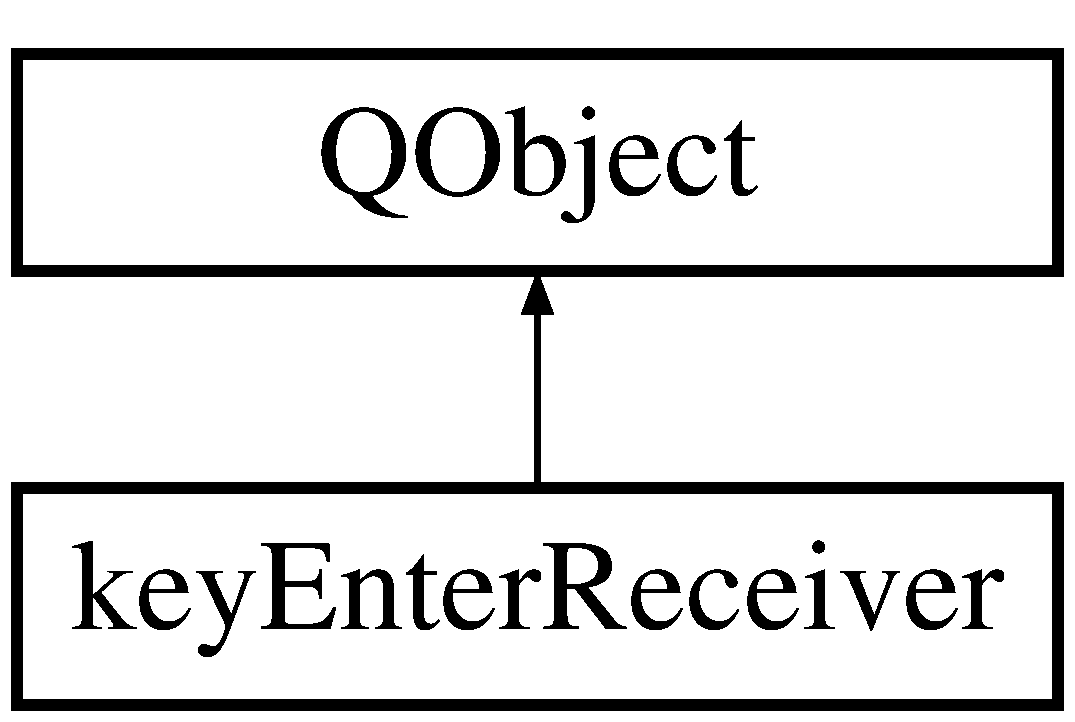
\includegraphics[height=2.000000cm]{classkeyEnterReceiver}
\end{center}
\end{figure}
\subsection*{Сигнали}
\begin{DoxyCompactItemize}
\item 
\hypertarget{classkeyEnterReceiver_af453b7b9a6b24cd91cf93fd3aabec434}{void {\bfseries enter\-Pressed} ()}\label{classkeyEnterReceiver_af453b7b9a6b24cd91cf93fd3aabec434}

\end{DoxyCompactItemize}
\subsection*{Загальнодоступні елементи}
\begin{DoxyCompactItemize}
\item 
\hypertarget{classkeyEnterReceiver_a36041eba96b5ddfc4118cfc6a9f2d252}{{\bfseries key\-Enter\-Receiver} (Q\-Object $\ast$parent=0)}\label{classkeyEnterReceiver_a36041eba96b5ddfc4118cfc6a9f2d252}

\end{DoxyCompactItemize}
\subsection*{Захищені елементи}
\begin{DoxyCompactItemize}
\item 
\hypertarget{classkeyEnterReceiver_af13c717478e5b9d91334c9829bc016e0}{bool {\bfseries event\-Filter} (Q\-Object $\ast$obj, Q\-Event $\ast$event)}\label{classkeyEnterReceiver_af13c717478e5b9d91334c9829bc016e0}

\end{DoxyCompactItemize}


Документація цих класів була створена з файлів\-:\begin{DoxyCompactItemize}
\item 
Recognitor/keyenterreceiver.\-h\item 
Recognitor/keyenterreceiver.\-cpp\item 
Recognitor/moc\-\_\-keyenterreceiver.\-cpp\end{DoxyCompactItemize}

\hypertarget{classUi_1_1MainWindow}{\section{Клас Ui\-:\-:Main\-Window}
\label{classUi_1_1MainWindow}\index{Ui\-::\-Main\-Window@{Ui\-::\-Main\-Window}}
}
Схема успадкувань для Ui\-:\-:Main\-Window\begin{figure}[H]
\begin{center}
\leavevmode
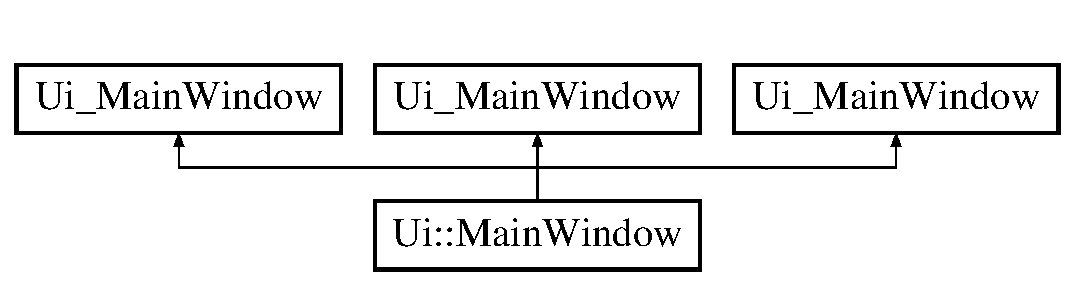
\includegraphics[height=2.000000cm]{classUi_1_1MainWindow}
\end{center}
\end{figure}
\subsection*{Additional Inherited Members}


Документація цього класу була створена з файлу\-:\begin{DoxyCompactItemize}
\item 
Recognitor-\/build-\/desktop-\/\-Qt\-\_\-4\-\_\-8\-\_\-3\-\_\-in\-\_\-\-P\-A\-T\-H\-\_\-\-\_\-\-System\-\_\-\-\_\-\-Release/ui\-\_\-mainwindow.\-h\end{DoxyCompactItemize}

\hypertarget{classMainWindow}{\section{Клас Main\-Window}
\label{classMainWindow}\index{Main\-Window@{Main\-Window}}
}
\subsection*{Загальнодоступні елементи}
\begin{DoxyCompactItemize}
\item 
\hypertarget{classMainWindow_a8b244be8b7b7db1b08de2a2acb9409db}{{\bfseries Main\-Window} (Q\-Widget $\ast$parent=0)}\label{classMainWindow_a8b244be8b7b7db1b08de2a2acb9409db}

\end{DoxyCompactItemize}
\subsection*{Приватні слоти}
\begin{DoxyCompactItemize}
\item 
\hypertarget{classMainWindow_ae0e46dc3da4ee07bf66e73e20300220c}{void {\bfseries on\-\_\-push\-Button\-\_\-2\-\_\-clicked} ()}\label{classMainWindow_ae0e46dc3da4ee07bf66e73e20300220c}

\item 
\hypertarget{classMainWindow_a4de79c63c7fa0b8d7c468ac71f20be81}{void {\bfseries on\-\_\-push\-Button\-\_\-clicked} ()}\label{classMainWindow_a4de79c63c7fa0b8d7c468ac71f20be81}

\end{DoxyCompactItemize}
\subsection*{Приватні дані}
\begin{DoxyCompactItemize}
\item 
\hypertarget{classMainWindow_a35466a70ed47252a0191168126a352a5}{\hyperlink{classUi_1_1MainWindow}{Ui\-::\-Main\-Window} $\ast$ {\bfseries ui}}\label{classMainWindow_a35466a70ed47252a0191168126a352a5}

\end{DoxyCompactItemize}


Документація цих класів була створена з файлів\-:\begin{DoxyCompactItemize}
\item 
Recognitor/\hyperlink{mainwindow_8h}{mainwindow.\-h}\item 
Recognitor/\hyperlink{mainwindow_8cpp}{mainwindow.\-cpp}\end{DoxyCompactItemize}

\hypertarget{classPacket}{\section{Клас Packet}
\label{classPacket}\index{Packet@{Packet}}
}
\subsection*{Загальнодоступні елементи}
\begin{DoxyCompactItemize}
\item 
\hypertarget{classPacket_a30fc0d2e5589228708582af6b5b2a576}{{\bfseries Packet} (\hyperlink{classPacket}{Packet} \&p)}\label{classPacket_a30fc0d2e5589228708582af6b5b2a576}

\item 
\hypertarget{classPacket_a3b5e228aeb6b3b4988f69433a9ccfb57}{{\bfseries Packet} (R\-Q\-T\-Y\-P\-E R\-E\-Q\-U\-E\-S\-T\-\_\-\-I\-D, int S\-E\-S\-S\-I\-O\-N\-\_\-\-I\-D, int S\-I\-Z\-E, char $\ast$D\-A\-T\-A)}\label{classPacket_a3b5e228aeb6b3b4988f69433a9ccfb57}

\item 
\hypertarget{classPacket_a0a267f964f5d9bf71159103eda50fbec}{Q\-Byte\-Array {\bfseries get\-Bytes} ()}\label{classPacket_a0a267f964f5d9bf71159103eda50fbec}

\item 
\hypertarget{classPacket_aeca5b2428ba736a24fe08c7322b74bb0}{\hyperlink{classPacket}{Packet} {\bfseries send} (Q\-String I\-P, int port)}\label{classPacket_aeca5b2428ba736a24fe08c7322b74bb0}

\end{DoxyCompactItemize}
\subsection*{Приватні дані}
\begin{DoxyCompactItemize}
\item 
\hypertarget{classPacket_a1e3e5174c14d3fa58d84e3449fbc8528}{R\-Q\-T\-Y\-P\-E {\bfseries R\-E\-Q\-U\-E\-S\-T\-\_\-\-I\-D}}\label{classPacket_a1e3e5174c14d3fa58d84e3449fbc8528}

\item 
\hypertarget{classPacket_ab961c50e0041597c29c52d1e397c5f91}{int {\bfseries S\-E\-S\-S\-I\-O\-N\-\_\-\-I\-D}}\label{classPacket_ab961c50e0041597c29c52d1e397c5f91}

\item 
\hypertarget{classPacket_a095ff3c0e41af547f0f7cc2464b0cb87}{int {\bfseries S\-I\-Z\-E}}\label{classPacket_a095ff3c0e41af547f0f7cc2464b0cb87}

\item 
\hypertarget{classPacket_abc0a29f961bdd40de882e39601884866}{char $\ast$ {\bfseries D\-A\-T\-A}}\label{classPacket_abc0a29f961bdd40de882e39601884866}

\end{DoxyCompactItemize}


Документація цих класів була створена з файлів\-:\begin{DoxyCompactItemize}
\item 
Recognitor/packet.\-h\item 
Recognitor/packet.\-cpp\end{DoxyCompactItemize}

\hypertarget{structqt__meta__stringdata__AdminScreen__t}{\section{Структура qt\-\_\-meta\-\_\-stringdata\-\_\-\-Admin\-Screen\-\_\-t}
\label{structqt__meta__stringdata__AdminScreen__t}\index{qt\-\_\-meta\-\_\-stringdata\-\_\-\-Admin\-Screen\-\_\-t@{qt\-\_\-meta\-\_\-stringdata\-\_\-\-Admin\-Screen\-\_\-t}}
}
\subsection*{Загальнодоступні атрибути}
\begin{DoxyCompactItemize}
\item 
\hypertarget{structqt__meta__stringdata__AdminScreen__t_af98accc03a243a18f8dabcb467dd0455}{Q\-Byte\-Array\-Data {\bfseries data} \mbox{[}6\mbox{]}}\label{structqt__meta__stringdata__AdminScreen__t_af98accc03a243a18f8dabcb467dd0455}

\item 
\hypertarget{structqt__meta__stringdata__AdminScreen__t_a4c6518f37b23904a10245d10516cc4e1}{char {\bfseries stringdata} \mbox{[}108\mbox{]}}\label{structqt__meta__stringdata__AdminScreen__t_a4c6518f37b23904a10245d10516cc4e1}

\end{DoxyCompactItemize}


Документація цієї структури була створена з файлу\-:\begin{DoxyCompactItemize}
\item 
Recognitor/moc\-\_\-adminscreen.\-cpp\end{DoxyCompactItemize}

\hypertarget{structqt__meta__stringdata__CameraCapture__t}{\section{Структура qt\-\_\-meta\-\_\-stringdata\-\_\-\-Camera\-Capture\-\_\-t}
\label{structqt__meta__stringdata__CameraCapture__t}\index{qt\-\_\-meta\-\_\-stringdata\-\_\-\-Camera\-Capture\-\_\-t@{qt\-\_\-meta\-\_\-stringdata\-\_\-\-Camera\-Capture\-\_\-t}}
}
\subsection*{Загальнодоступні атрибути}
\begin{DoxyCompactItemize}
\item 
\hypertarget{structqt__meta__stringdata__CameraCapture__t_a0a501428764d9a198399568bd518a278}{Q\-Byte\-Array\-Data {\bfseries data} \mbox{[}6\mbox{]}}\label{structqt__meta__stringdata__CameraCapture__t_a0a501428764d9a198399568bd518a278}

\item 
\hypertarget{structqt__meta__stringdata__CameraCapture__t_acf4762e4529c8b66d172c23138da6344}{char {\bfseries stringdata} \mbox{[}45\mbox{]}}\label{structqt__meta__stringdata__CameraCapture__t_acf4762e4529c8b66d172c23138da6344}

\end{DoxyCompactItemize}


Документація цієї структури була створена з файлу\-:\begin{DoxyCompactItemize}
\item 
Recognitor/moc\-\_\-cameracapture.\-cpp\end{DoxyCompactItemize}

\hypertarget{structqt__meta__stringdata__ExUserScreen__t}{\section{Структура qt\-\_\-meta\-\_\-stringdata\-\_\-\-Ex\-User\-Screen\-\_\-t}
\label{structqt__meta__stringdata__ExUserScreen__t}\index{qt\-\_\-meta\-\_\-stringdata\-\_\-\-Ex\-User\-Screen\-\_\-t@{qt\-\_\-meta\-\_\-stringdata\-\_\-\-Ex\-User\-Screen\-\_\-t}}
}
\subsection*{Загальнодоступні атрибути}
\begin{DoxyCompactItemize}
\item 
\hypertarget{structqt__meta__stringdata__ExUserScreen__t_a85a59682b5504e781fc2f64b50597d59}{Q\-Byte\-Array\-Data {\bfseries data} \mbox{[}12\mbox{]}}\label{structqt__meta__stringdata__ExUserScreen__t_a85a59682b5504e781fc2f64b50597d59}

\item 
\hypertarget{structqt__meta__stringdata__ExUserScreen__t_a5a72f104d835db06eca6b09b280b10ce}{char {\bfseries stringdata} \mbox{[}138\mbox{]}}\label{structqt__meta__stringdata__ExUserScreen__t_a5a72f104d835db06eca6b09b280b10ce}

\end{DoxyCompactItemize}


Документація цієї структури була створена з файлу\-:\begin{DoxyCompactItemize}
\item 
Recognitor/moc\-\_\-exuserscreen.\-cpp\end{DoxyCompactItemize}

\hypertarget{structqt__meta__stringdata__GoodsMgmtScreen__t}{\section{Структура qt\-\_\-meta\-\_\-stringdata\-\_\-\-Goods\-Mgmt\-Screen\-\_\-t}
\label{structqt__meta__stringdata__GoodsMgmtScreen__t}\index{qt\-\_\-meta\-\_\-stringdata\-\_\-\-Goods\-Mgmt\-Screen\-\_\-t@{qt\-\_\-meta\-\_\-stringdata\-\_\-\-Goods\-Mgmt\-Screen\-\_\-t}}
}
\subsection*{Загальнодоступні атрибути}
\begin{DoxyCompactItemize}
\item 
\hypertarget{structqt__meta__stringdata__GoodsMgmtScreen__t_a1e2034ea98f4dca1030329e201d0b1c6}{Q\-Byte\-Array\-Data {\bfseries data} \mbox{[}6\mbox{]}}\label{structqt__meta__stringdata__GoodsMgmtScreen__t_a1e2034ea98f4dca1030329e201d0b1c6}

\item 
\hypertarget{structqt__meta__stringdata__GoodsMgmtScreen__t_aaaef1513790130b3b88a004f667480ec}{char {\bfseries stringdata} \mbox{[}112\mbox{]}}\label{structqt__meta__stringdata__GoodsMgmtScreen__t_aaaef1513790130b3b88a004f667480ec}

\end{DoxyCompactItemize}


Документація цієї структури була створена з файлу\-:\begin{DoxyCompactItemize}
\item 
Recognitor/moc\-\_\-goodsmgmtscreen.\-cpp\end{DoxyCompactItemize}

\hypertarget{structqt__meta__stringdata__keyEnterReceiver__t}{\section{Структура qt\-\_\-meta\-\_\-stringdata\-\_\-key\-Enter\-Receiver\-\_\-t}
\label{structqt__meta__stringdata__keyEnterReceiver__t}\index{qt\-\_\-meta\-\_\-stringdata\-\_\-key\-Enter\-Receiver\-\_\-t@{qt\-\_\-meta\-\_\-stringdata\-\_\-key\-Enter\-Receiver\-\_\-t}}
}
\subsection*{Загальнодоступні атрибути}
\begin{DoxyCompactItemize}
\item 
\hypertarget{structqt__meta__stringdata__keyEnterReceiver__t_a9e2ca77621768144ceb41c6d84f1f16a}{Q\-Byte\-Array\-Data {\bfseries data} \mbox{[}3\mbox{]}}\label{structqt__meta__stringdata__keyEnterReceiver__t_a9e2ca77621768144ceb41c6d84f1f16a}

\item 
\hypertarget{structqt__meta__stringdata__keyEnterReceiver__t_a4956864d5080e03e51b6d137cd787215}{char {\bfseries stringdata} \mbox{[}32\mbox{]}}\label{structqt__meta__stringdata__keyEnterReceiver__t_a4956864d5080e03e51b6d137cd787215}

\end{DoxyCompactItemize}


Документація цієї структури була створена з файлу\-:\begin{DoxyCompactItemize}
\item 
Recognitor/moc\-\_\-keyenterreceiver.\-cpp\end{DoxyCompactItemize}

\hypertarget{structqt__meta__stringdata__MainWindow__t}{\section{Структура qt\-\_\-meta\-\_\-stringdata\-\_\-\-Main\-Window\-\_\-t}
\label{structqt__meta__stringdata__MainWindow__t}\index{qt\-\_\-meta\-\_\-stringdata\-\_\-\-Main\-Window\-\_\-t@{qt\-\_\-meta\-\_\-stringdata\-\_\-\-Main\-Window\-\_\-t}}
}
\subsection*{Загальнодоступні атрибути}
\begin{DoxyCompactItemize}
\item 
\hypertarget{structqt__meta__stringdata__MainWindow__t_a332d7fa058028f7613b5ba68abb5a7fe}{Q\-Byte\-Array\-Data {\bfseries data} \mbox{[}4\mbox{]}}\label{structqt__meta__stringdata__MainWindow__t_a332d7fa058028f7613b5ba68abb5a7fe}

\item 
\hypertarget{structqt__meta__stringdata__MainWindow__t_a1f75f6e6169dcfddb4a6e5701e72456e}{char {\bfseries stringdata} \mbox{[}59\mbox{]}}\label{structqt__meta__stringdata__MainWindow__t_a1f75f6e6169dcfddb4a6e5701e72456e}

\end{DoxyCompactItemize}


Документація цієї структури була створена з файлу\-:\begin{DoxyCompactItemize}
\item 
Recognitor/moc\-\_\-mainwindow.\-cpp\end{DoxyCompactItemize}

\hypertarget{structqt__meta__stringdata__UserScreen__t}{\section{Структура qt\-\_\-meta\-\_\-stringdata\-\_\-\-User\-Screen\-\_\-t}
\label{structqt__meta__stringdata__UserScreen__t}\index{qt\-\_\-meta\-\_\-stringdata\-\_\-\-User\-Screen\-\_\-t@{qt\-\_\-meta\-\_\-stringdata\-\_\-\-User\-Screen\-\_\-t}}
}
\subsection*{Загальнодоступні атрибути}
\begin{DoxyCompactItemize}
\item 
\hypertarget{structqt__meta__stringdata__UserScreen__t_acd72156d5b155fea32a0248c1724c4d1}{Q\-Byte\-Array\-Data {\bfseries data} \mbox{[}11\mbox{]}}\label{structqt__meta__stringdata__UserScreen__t_acd72156d5b155fea32a0248c1724c4d1}

\item 
\hypertarget{structqt__meta__stringdata__UserScreen__t_ace3d7ec5b8f13f42a1b256620a22e71f}{char {\bfseries stringdata} \mbox{[}112\mbox{]}}\label{structqt__meta__stringdata__UserScreen__t_ace3d7ec5b8f13f42a1b256620a22e71f}

\end{DoxyCompactItemize}


Документація цієї структури була створена з файлу\-:\begin{DoxyCompactItemize}
\item 
Recognitor/moc\-\_\-userscreen.\-cpp\end{DoxyCompactItemize}

\hypertarget{classUi__AdminScreen}{\section{Клас Ui\-\_\-\-Admin\-Screen}
\label{classUi__AdminScreen}\index{Ui\-\_\-\-Admin\-Screen@{Ui\-\_\-\-Admin\-Screen}}
}
Схема успадкувань для Ui\-\_\-\-Admin\-Screen\begin{figure}[H]
\begin{center}
\leavevmode
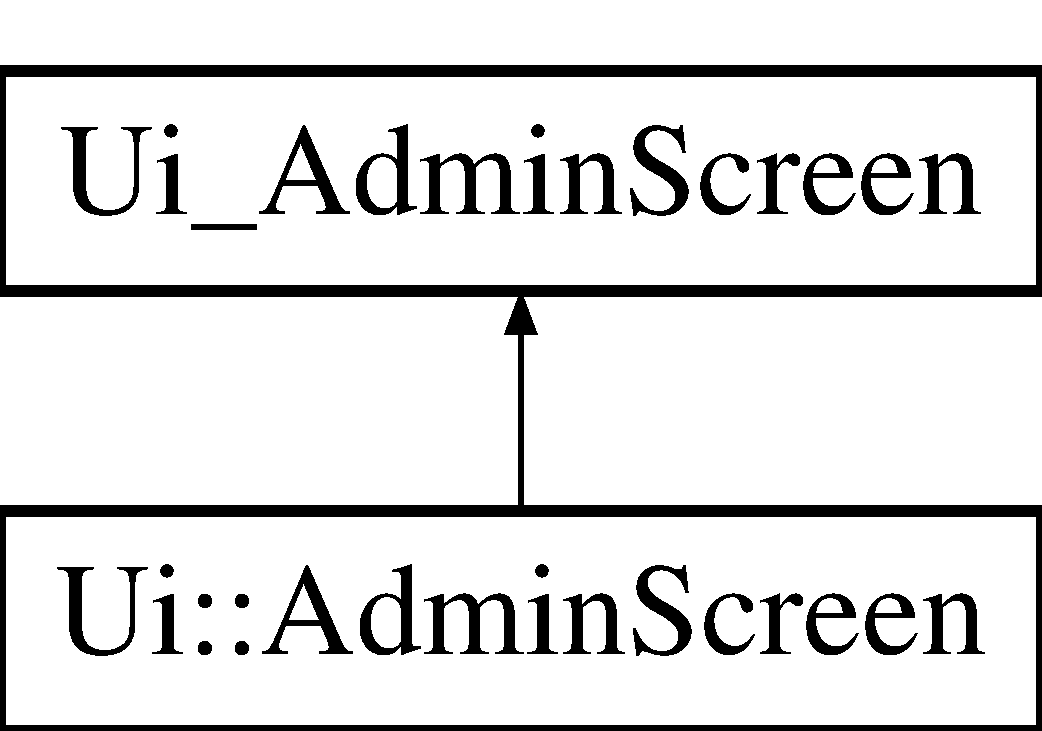
\includegraphics[height=2.000000cm]{classUi__AdminScreen}
\end{center}
\end{figure}
\subsection*{Загальнодоступні елементи}
\begin{DoxyCompactItemize}
\item 
\hypertarget{classUi__AdminScreen_a0a67dc309a34eb0240dedbd00754fd7e}{void {\bfseries setup\-Ui} (Q\-Main\-Window $\ast$\hyperlink{classAdminScreen}{Admin\-Screen})}\label{classUi__AdminScreen_a0a67dc309a34eb0240dedbd00754fd7e}

\item 
\hypertarget{classUi__AdminScreen_aa6891d66f0e464aa293fd66b1330cc19}{void {\bfseries retranslate\-Ui} (Q\-Main\-Window $\ast$\hyperlink{classAdminScreen}{Admin\-Screen})}\label{classUi__AdminScreen_aa6891d66f0e464aa293fd66b1330cc19}

\end{DoxyCompactItemize}
\subsection*{Загальнодоступні атрибути}
\begin{DoxyCompactItemize}
\item 
\hypertarget{classUi__AdminScreen_ab66473b046e698cd8090c3fa0fa404f8}{Q\-Widget $\ast$ {\bfseries centralwidget}}\label{classUi__AdminScreen_ab66473b046e698cd8090c3fa0fa404f8}

\item 
\hypertarget{classUi__AdminScreen_ad315d893b5b5b0f1ddc07e3015826af9}{Q\-Table\-View $\ast$ {\bfseries table\-View}}\label{classUi__AdminScreen_ad315d893b5b5b0f1ddc07e3015826af9}

\item 
\hypertarget{classUi__AdminScreen_a1212e3eec1524e8796bc5477a696c920}{Q\-Widget $\ast$ {\bfseries widget}}\label{classUi__AdminScreen_a1212e3eec1524e8796bc5477a696c920}

\item 
\hypertarget{classUi__AdminScreen_a35e2f0ce11c816c94537e0cc0e82802a}{Q\-V\-Box\-Layout $\ast$ {\bfseries vertical\-Layout}}\label{classUi__AdminScreen_a35e2f0ce11c816c94537e0cc0e82802a}

\item 
\hypertarget{classUi__AdminScreen_a68c1187df54f74e05838aa4504ffedf5}{Q\-Push\-Button $\ast$ {\bfseries push\-Button\-\_\-2}}\label{classUi__AdminScreen_a68c1187df54f74e05838aa4504ffedf5}

\item 
\hypertarget{classUi__AdminScreen_a676124dea795926160a979a358e5d675}{Q\-Push\-Button $\ast$ {\bfseries push\-Button\-\_\-3}}\label{classUi__AdminScreen_a676124dea795926160a979a358e5d675}

\item 
\hypertarget{classUi__AdminScreen_a6ff6389f23502818e00c3e74b04de510}{Q\-Push\-Button $\ast$ {\bfseries push\-Button\-\_\-4}}\label{classUi__AdminScreen_a6ff6389f23502818e00c3e74b04de510}

\item 
\hypertarget{classUi__AdminScreen_abaf9409db469e4b7edcb7701b3f4b7f4}{Q\-Spacer\-Item $\ast$ {\bfseries vertical\-Spacer}}\label{classUi__AdminScreen_abaf9409db469e4b7edcb7701b3f4b7f4}

\item 
\hypertarget{classUi__AdminScreen_a5e92b9e0a9297641f89d393e1e31ba3f}{Q\-Push\-Button $\ast$ {\bfseries push\-Button}}\label{classUi__AdminScreen_a5e92b9e0a9297641f89d393e1e31ba3f}

\end{DoxyCompactItemize}


Документація цього класу була створена з файлу\-:\begin{DoxyCompactItemize}
\item 
Recognitor-\/build-\/desktop-\/\-Qt\-\_\-4\-\_\-8\-\_\-3\-\_\-in\-\_\-\-P\-A\-T\-H\-\_\-\-\_\-\-System\-\_\-\-\_\-\-Release/ui\-\_\-adminscreen.\-h\end{DoxyCompactItemize}

\hypertarget{classUi__ExUserScreen}{\section{Клас Ui\-\_\-\-Ex\-User\-Screen}
\label{classUi__ExUserScreen}\index{Ui\-\_\-\-Ex\-User\-Screen@{Ui\-\_\-\-Ex\-User\-Screen}}
}
Схема успадкувань для Ui\-\_\-\-Ex\-User\-Screen\begin{figure}[H]
\begin{center}
\leavevmode
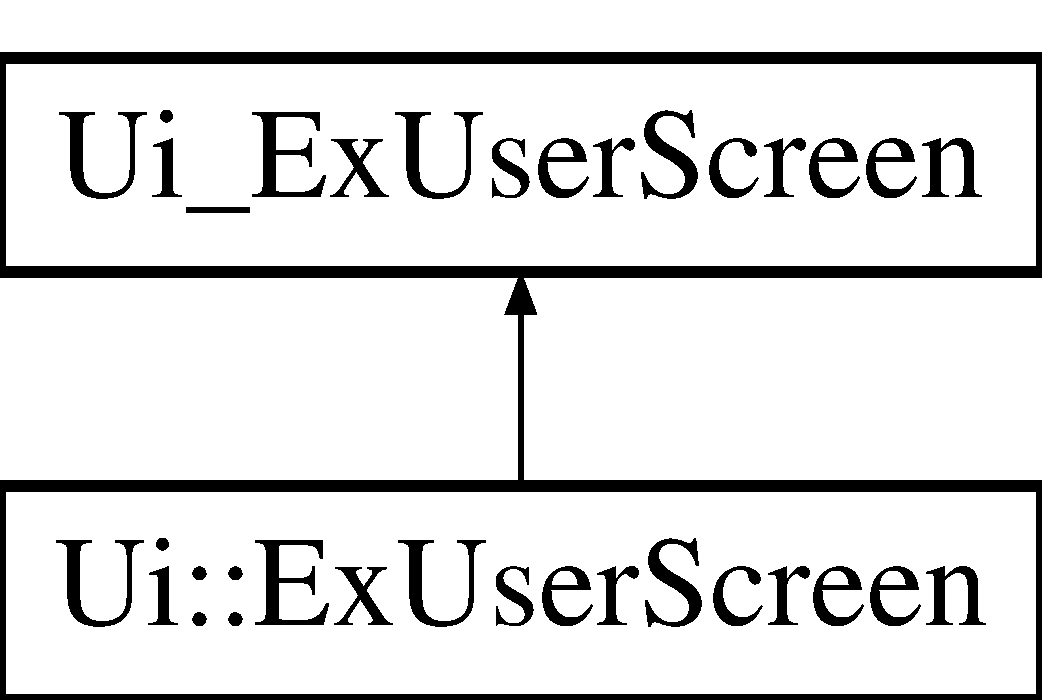
\includegraphics[height=2.000000cm]{classUi__ExUserScreen}
\end{center}
\end{figure}
\subsection*{Загальнодоступні елементи}
\begin{DoxyCompactItemize}
\item 
\hypertarget{classUi__ExUserScreen_a166ae2661d465ac77a86487c3a394fcb}{void {\bfseries setup\-Ui} (Q\-Main\-Window $\ast$\hyperlink{classExUserScreen}{Ex\-User\-Screen})}\label{classUi__ExUserScreen_a166ae2661d465ac77a86487c3a394fcb}

\item 
\hypertarget{classUi__ExUserScreen_a4cc3648836b29adf36758dcff29d6761}{void {\bfseries retranslate\-Ui} (Q\-Main\-Window $\ast$\hyperlink{classExUserScreen}{Ex\-User\-Screen})}\label{classUi__ExUserScreen_a4cc3648836b29adf36758dcff29d6761}

\end{DoxyCompactItemize}
\subsection*{Загальнодоступні атрибути}
\begin{DoxyCompactItemize}
\item 
\hypertarget{classUi__ExUserScreen_a2a99013ef3fceba6fc51ae3cc2d7b2e1}{Q\-Widget $\ast$ {\bfseries centralwidget}}\label{classUi__ExUserScreen_a2a99013ef3fceba6fc51ae3cc2d7b2e1}

\item 
\hypertarget{classUi__ExUserScreen_a898af8b981323f54c0ecd7e5bedb2f4b}{Q\-Widget $\ast$ {\bfseries layout\-Widget}}\label{classUi__ExUserScreen_a898af8b981323f54c0ecd7e5bedb2f4b}

\item 
\hypertarget{classUi__ExUserScreen_a7acd541ca534e13a6926a4f29e643d76}{Q\-V\-Box\-Layout $\ast$ {\bfseries vertical\-Layout}}\label{classUi__ExUserScreen_a7acd541ca534e13a6926a4f29e643d76}

\item 
\hypertarget{classUi__ExUserScreen_aa37b97327956d99f6a3bddb595c9af45}{Q\-Graphics\-View $\ast$ {\bfseries graphics\-View}}\label{classUi__ExUserScreen_aa37b97327956d99f6a3bddb595c9af45}

\item 
\hypertarget{classUi__ExUserScreen_ab3f8745ecef533e45add685a3a0e43d5}{Q\-H\-Box\-Layout $\ast$ {\bfseries horizontal\-Layout\-\_\-3}}\label{classUi__ExUserScreen_ab3f8745ecef533e45add685a3a0e43d5}

\item 
\hypertarget{classUi__ExUserScreen_ae94f4b8796e08e30ccd807e67009f63d}{Q\-Spacer\-Item $\ast$ {\bfseries horizontal\-Spacer\-\_\-2}}\label{classUi__ExUserScreen_ae94f4b8796e08e30ccd807e67009f63d}

\item 
\hypertarget{classUi__ExUserScreen_afba2a4123fe138f23304a56a1b0befff}{Q\-Push\-Button $\ast$ {\bfseries push\-Button}}\label{classUi__ExUserScreen_afba2a4123fe138f23304a56a1b0befff}

\item 
\hypertarget{classUi__ExUserScreen_afa1e70d1828cd20eac01382328721f6f}{Q\-Spacer\-Item $\ast$ {\bfseries horizontal\-Spacer}}\label{classUi__ExUserScreen_afa1e70d1828cd20eac01382328721f6f}

\item 
\hypertarget{classUi__ExUserScreen_a903a62e821583de883b0b1192b7be15f}{Q\-H\-Box\-Layout $\ast$ {\bfseries horizontal\-Layout\-\_\-4}}\label{classUi__ExUserScreen_a903a62e821583de883b0b1192b7be15f}

\item 
\hypertarget{classUi__ExUserScreen_a05799742a0b74c8058aebabac80a4943}{Q\-Label $\ast$ {\bfseries label}}\label{classUi__ExUserScreen_a05799742a0b74c8058aebabac80a4943}

\item 
\hypertarget{classUi__ExUserScreen_a8e000c8945bfbbd9e91a1001f97ce6b0}{Q\-Spin\-Box $\ast$ {\bfseries spin\-Box}}\label{classUi__ExUserScreen_a8e000c8945bfbbd9e91a1001f97ce6b0}

\item 
\hypertarget{classUi__ExUserScreen_ab3f6f286a82c961f46f54918f346d7b3}{Q\-Label $\ast$ {\bfseries label\-\_\-2}}\label{classUi__ExUserScreen_ab3f6f286a82c961f46f54918f346d7b3}

\item 
\hypertarget{classUi__ExUserScreen_abc80fe6702095d4adbe13f40207bcfc3}{Q\-H\-Box\-Layout $\ast$ {\bfseries horizontal\-Layout}}\label{classUi__ExUserScreen_abc80fe6702095d4adbe13f40207bcfc3}

\item 
\hypertarget{classUi__ExUserScreen_a9e0be9622eeeefbd45b87703b3968086}{Q\-Spacer\-Item $\ast$ {\bfseries horizontal\-Spacer\-\_\-5}}\label{classUi__ExUserScreen_a9e0be9622eeeefbd45b87703b3968086}

\item 
\hypertarget{classUi__ExUserScreen_aac92023264e115d0601eaee5fae09ddf}{Q\-Push\-Button $\ast$ {\bfseries push\-Button\-\_\-3}}\label{classUi__ExUserScreen_aac92023264e115d0601eaee5fae09ddf}

\item 
\hypertarget{classUi__ExUserScreen_ad388fc01774a6ad9100914452d5ba130}{Q\-Spacer\-Item $\ast$ {\bfseries horizontal\-Spacer\-\_\-6}}\label{classUi__ExUserScreen_ad388fc01774a6ad9100914452d5ba130}

\item 
\hypertarget{classUi__ExUserScreen_a2a9ce1e768cc5cbd28de9d55c15f8018}{Q\-H\-Box\-Layout $\ast$ {\bfseries horizontal\-Layout\-\_\-2}}\label{classUi__ExUserScreen_a2a9ce1e768cc5cbd28de9d55c15f8018}

\item 
\hypertarget{classUi__ExUserScreen_a085949386f33d45e979c5d82734efd24}{Q\-Spacer\-Item $\ast$ {\bfseries horizontal\-Spacer\-\_\-3}}\label{classUi__ExUserScreen_a085949386f33d45e979c5d82734efd24}

\item 
\hypertarget{classUi__ExUserScreen_a224a14a86010a782348c2fcc14ec12b9}{Q\-Push\-Button $\ast$ {\bfseries push\-Button\-\_\-2}}\label{classUi__ExUserScreen_a224a14a86010a782348c2fcc14ec12b9}

\item 
\hypertarget{classUi__ExUserScreen_a310830e48e61fcd344d64290e8802c25}{Q\-Spacer\-Item $\ast$ {\bfseries horizontal\-Spacer\-\_\-4}}\label{classUi__ExUserScreen_a310830e48e61fcd344d64290e8802c25}

\end{DoxyCompactItemize}


Документація цього класу була створена з файлу\-:\begin{DoxyCompactItemize}
\item 
Recognitor-\/build-\/desktop-\/\-Qt\-\_\-4\-\_\-8\-\_\-3\-\_\-in\-\_\-\-P\-A\-T\-H\-\_\-\-\_\-\-System\-\_\-\-\_\-\-Release/ui\-\_\-exuserscreen.\-h\end{DoxyCompactItemize}

\hypertarget{classUi__GoodsMgmtScreen}{\section{Клас Ui\-\_\-\-Goods\-Mgmt\-Screen}
\label{classUi__GoodsMgmtScreen}\index{Ui\-\_\-\-Goods\-Mgmt\-Screen@{Ui\-\_\-\-Goods\-Mgmt\-Screen}}
}
Схема успадкувань для Ui\-\_\-\-Goods\-Mgmt\-Screen\begin{figure}[H]
\begin{center}
\leavevmode
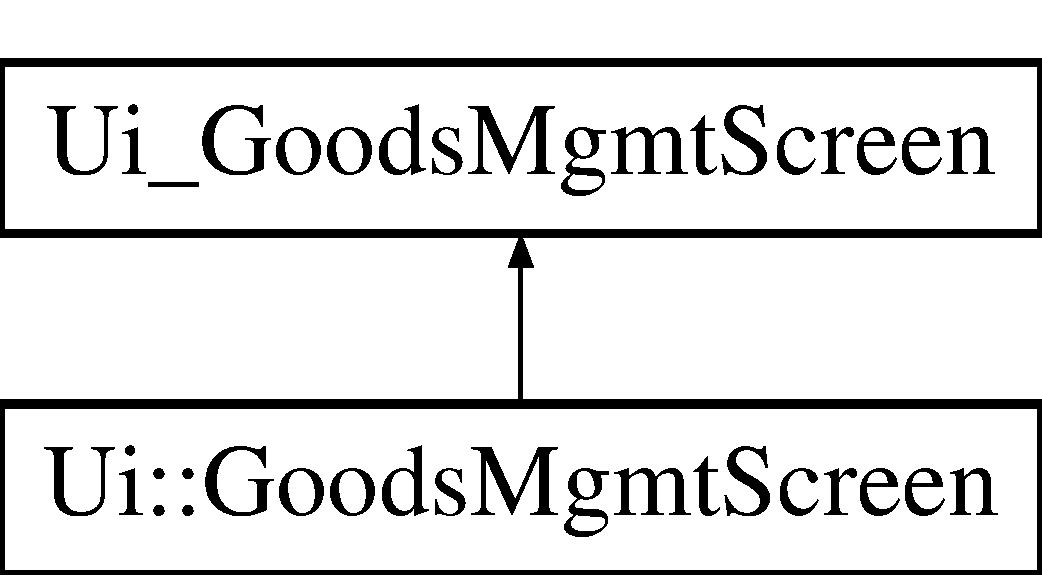
\includegraphics[height=2.000000cm]{classUi__GoodsMgmtScreen}
\end{center}
\end{figure}
\subsection*{Загальнодоступні елементи}
\begin{DoxyCompactItemize}
\item 
\hypertarget{classUi__GoodsMgmtScreen_a8baf991b8f140c374f26406651bf3244}{void {\bfseries setup\-Ui} (Q\-Main\-Window $\ast$\hyperlink{classGoodsMgmtScreen}{Goods\-Mgmt\-Screen})}\label{classUi__GoodsMgmtScreen_a8baf991b8f140c374f26406651bf3244}

\item 
\hypertarget{classUi__GoodsMgmtScreen_a0cfda36456b30c0be0117295991c9a46}{void {\bfseries retranslate\-Ui} (Q\-Main\-Window $\ast$\hyperlink{classGoodsMgmtScreen}{Goods\-Mgmt\-Screen})}\label{classUi__GoodsMgmtScreen_a0cfda36456b30c0be0117295991c9a46}

\item 
\hypertarget{classUi__GoodsMgmtScreen_a8baf991b8f140c374f26406651bf3244}{void {\bfseries setup\-Ui} (Q\-Main\-Window $\ast$\hyperlink{classGoodsMgmtScreen}{Goods\-Mgmt\-Screen})}\label{classUi__GoodsMgmtScreen_a8baf991b8f140c374f26406651bf3244}

\item 
\hypertarget{classUi__GoodsMgmtScreen_a0cfda36456b30c0be0117295991c9a46}{void {\bfseries retranslate\-Ui} (Q\-Main\-Window $\ast$\hyperlink{classGoodsMgmtScreen}{Goods\-Mgmt\-Screen})}\label{classUi__GoodsMgmtScreen_a0cfda36456b30c0be0117295991c9a46}

\item 
\hypertarget{classUi__GoodsMgmtScreen_a8baf991b8f140c374f26406651bf3244}{void {\bfseries setup\-Ui} (Q\-Main\-Window $\ast$\hyperlink{classGoodsMgmtScreen}{Goods\-Mgmt\-Screen})}\label{classUi__GoodsMgmtScreen_a8baf991b8f140c374f26406651bf3244}

\item 
\hypertarget{classUi__GoodsMgmtScreen_a0cfda36456b30c0be0117295991c9a46}{void {\bfseries retranslate\-Ui} (Q\-Main\-Window $\ast$\hyperlink{classGoodsMgmtScreen}{Goods\-Mgmt\-Screen})}\label{classUi__GoodsMgmtScreen_a0cfda36456b30c0be0117295991c9a46}

\end{DoxyCompactItemize}
\subsection*{Загальнодоступні атрибути}
\begin{DoxyCompactItemize}
\item 
\hypertarget{classUi__GoodsMgmtScreen_a51b13e31b350281491052f3d5971ae60}{Q\-Widget $\ast$ {\bfseries centralwidget}}\label{classUi__GoodsMgmtScreen_a51b13e31b350281491052f3d5971ae60}

\item 
\hypertarget{classUi__GoodsMgmtScreen_a886d6c0b18e00ae84565e97d7e7a4315}{Q\-Widget $\ast$ {\bfseries widget}}\label{classUi__GoodsMgmtScreen_a886d6c0b18e00ae84565e97d7e7a4315}

\item 
\hypertarget{classUi__GoodsMgmtScreen_aeae0577797c24c57d957d776a66362ad}{Q\-H\-Box\-Layout $\ast$ {\bfseries horizontal\-Layout}}\label{classUi__GoodsMgmtScreen_aeae0577797c24c57d957d776a66362ad}

\item 
\hypertarget{classUi__GoodsMgmtScreen_a15a34ca1bb6de6ee947406d7e81aea7e}{Q\-Table\-View $\ast$ {\bfseries table\-View}}\label{classUi__GoodsMgmtScreen_a15a34ca1bb6de6ee947406d7e81aea7e}

\item 
\hypertarget{classUi__GoodsMgmtScreen_aa94a6f911507c470f171ca535d86e267}{Q\-Spacer\-Item $\ast$ {\bfseries horizontal\-Spacer\-\_\-2}}\label{classUi__GoodsMgmtScreen_aa94a6f911507c470f171ca535d86e267}

\item 
\hypertarget{classUi__GoodsMgmtScreen_a6203c3363ae73c2a34b473fad6f85df5}{Q\-V\-Box\-Layout $\ast$ {\bfseries vertical\-Layout}}\label{classUi__GoodsMgmtScreen_a6203c3363ae73c2a34b473fad6f85df5}

\item 
\hypertarget{classUi__GoodsMgmtScreen_a7d598759631c0e67beb8ba2546b475ce}{Q\-Spacer\-Item $\ast$ {\bfseries vertical\-Spacer\-\_\-2}}\label{classUi__GoodsMgmtScreen_a7d598759631c0e67beb8ba2546b475ce}

\item 
\hypertarget{classUi__GoodsMgmtScreen_a6d94c562fc4812065faf476820c604e0}{Q\-Push\-Button $\ast$ {\bfseries push\-Button}}\label{classUi__GoodsMgmtScreen_a6d94c562fc4812065faf476820c604e0}

\item 
\hypertarget{classUi__GoodsMgmtScreen_a65afa4141945ad4421e90546ca5ba25b}{Q\-Push\-Button $\ast$ {\bfseries push\-Button\-\_\-2}}\label{classUi__GoodsMgmtScreen_a65afa4141945ad4421e90546ca5ba25b}

\item 
\hypertarget{classUi__GoodsMgmtScreen_ae22ee60fef7839256b0d27feea4da8cb}{Q\-Push\-Button $\ast$ {\bfseries push\-Button\-\_\-3}}\label{classUi__GoodsMgmtScreen_ae22ee60fef7839256b0d27feea4da8cb}

\item 
\hypertarget{classUi__GoodsMgmtScreen_ab186a744bf6fccf3bf1365eeab01d686}{Q\-Spacer\-Item $\ast$ {\bfseries vertical\-Spacer}}\label{classUi__GoodsMgmtScreen_ab186a744bf6fccf3bf1365eeab01d686}

\item 
\hypertarget{classUi__GoodsMgmtScreen_a737f8c6f826a2506dd5ababe3b8f2390}{Q\-Push\-Button $\ast$ {\bfseries push\-Button\-\_\-4}}\label{classUi__GoodsMgmtScreen_a737f8c6f826a2506dd5ababe3b8f2390}

\item 
\hypertarget{classUi__GoodsMgmtScreen_a64dd0fe73061c502f7c3dc84eaf0116e}{Q\-Spacer\-Item $\ast$ {\bfseries vertical\-Spacer\-\_\-3}}\label{classUi__GoodsMgmtScreen_a64dd0fe73061c502f7c3dc84eaf0116e}

\item 
\hypertarget{classUi__GoodsMgmtScreen_aeb1cd255574a0a7fdc77fc423d826e55}{Q\-Spacer\-Item $\ast$ {\bfseries horizontal\-Spacer}}\label{classUi__GoodsMgmtScreen_aeb1cd255574a0a7fdc77fc423d826e55}

\end{DoxyCompactItemize}


Документація цього класу була створена з файлу\-:\begin{DoxyCompactItemize}
\item 
Recognitor/ui\-\_\-goodsmgmtscreen.\-h\end{DoxyCompactItemize}

\hypertarget{classUi__MainWindow}{\section{Клас Ui\-\_\-\-Main\-Window}
\label{classUi__MainWindow}\index{Ui\-\_\-\-Main\-Window@{Ui\-\_\-\-Main\-Window}}
}
Схема успадкувань для Ui\-\_\-\-Main\-Window\begin{figure}[H]
\begin{center}
\leavevmode
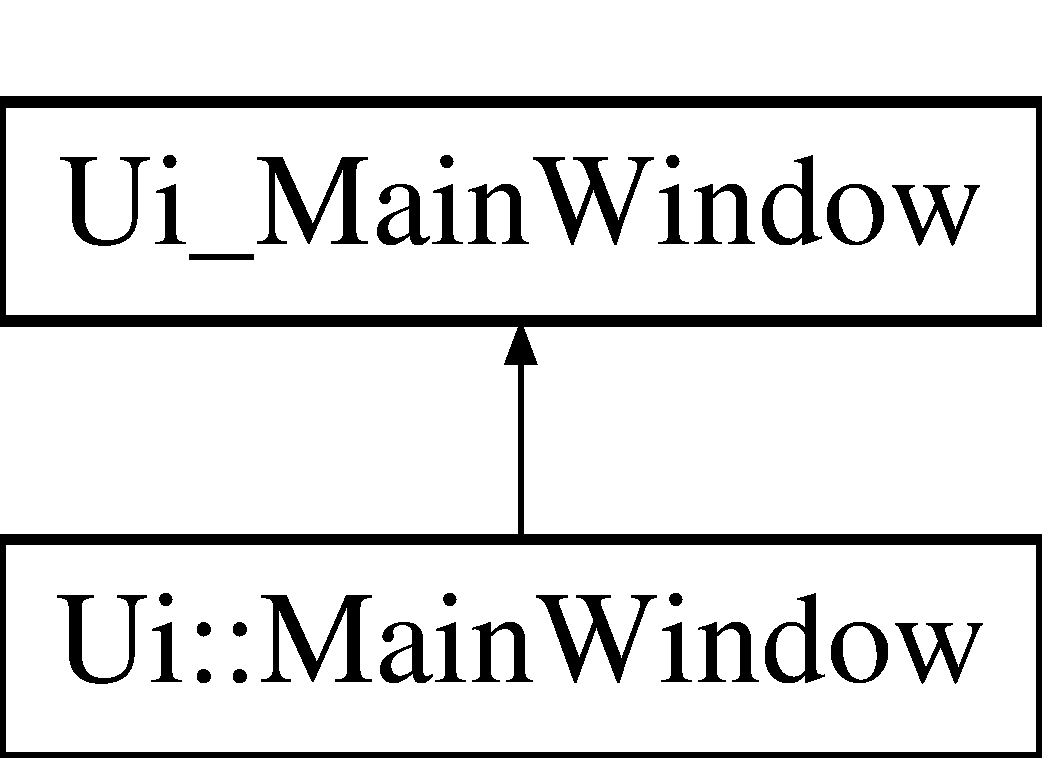
\includegraphics[height=2.000000cm]{classUi__MainWindow}
\end{center}
\end{figure}
\subsection*{Загальнодоступні елементи}
\begin{DoxyCompactItemize}
\item 
\hypertarget{classUi__MainWindow_acf4a0872c4c77d8f43a2ec66ed849b58}{void {\bfseries setup\-Ui} (Q\-Main\-Window $\ast$\hyperlink{classMainWindow}{Main\-Window})}\label{classUi__MainWindow_acf4a0872c4c77d8f43a2ec66ed849b58}

\item 
\hypertarget{classUi__MainWindow_a097dd160c3534a204904cb374412c618}{void {\bfseries retranslate\-Ui} (Q\-Main\-Window $\ast$\hyperlink{classMainWindow}{Main\-Window})}\label{classUi__MainWindow_a097dd160c3534a204904cb374412c618}

\end{DoxyCompactItemize}
\subsection*{Загальнодоступні атрибути}
\begin{DoxyCompactItemize}
\item 
\hypertarget{classUi__MainWindow_a356f1cf3ebda15f1fac59467ee081b74}{Q\-Widget $\ast$ {\bfseries centralwidget}}\label{classUi__MainWindow_a356f1cf3ebda15f1fac59467ee081b74}

\item 
\hypertarget{classUi__MainWindow_ab96ab0f0578098521fa69a75aa5cdde8}{Q\-Widget $\ast$ {\bfseries layout\-Widget}}\label{classUi__MainWindow_ab96ab0f0578098521fa69a75aa5cdde8}

\item 
\hypertarget{classUi__MainWindow_aecd96a04789fcfec3f98d80390ad8184}{Q\-V\-Box\-Layout $\ast$ {\bfseries vertical\-Layout}}\label{classUi__MainWindow_aecd96a04789fcfec3f98d80390ad8184}

\item 
\hypertarget{classUi__MainWindow_a0376fd90247280e7c7957cc70628708c}{Q\-Label $\ast$ {\bfseries label\-\_\-3}}\label{classUi__MainWindow_a0376fd90247280e7c7957cc70628708c}

\item 
\hypertarget{classUi__MainWindow_acd6fdc9ebacc4b25b834162380d75ce8}{Q\-H\-Box\-Layout $\ast$ {\bfseries horizontal\-Layout}}\label{classUi__MainWindow_acd6fdc9ebacc4b25b834162380d75ce8}

\item 
\hypertarget{classUi__MainWindow_ad9c89133780f28e6efa2ec17ceb9cff5}{Q\-Label $\ast$ {\bfseries label}}\label{classUi__MainWindow_ad9c89133780f28e6efa2ec17ceb9cff5}

\item 
\hypertarget{classUi__MainWindow_a7a5b9a4633d64f502ce81da3202d828c}{Q\-Line\-Edit $\ast$ {\bfseries line\-Edit}}\label{classUi__MainWindow_a7a5b9a4633d64f502ce81da3202d828c}

\item 
\hypertarget{classUi__MainWindow_a80867018070156432923d0266cc9fe25}{Q\-H\-Box\-Layout $\ast$ {\bfseries horizontal\-Layout\-\_\-2}}\label{classUi__MainWindow_a80867018070156432923d0266cc9fe25}

\item 
\hypertarget{classUi__MainWindow_a2e2516d755e4dd53fc905dabddf2738a}{Q\-Label $\ast$ {\bfseries label\-\_\-2}}\label{classUi__MainWindow_a2e2516d755e4dd53fc905dabddf2738a}

\item 
\hypertarget{classUi__MainWindow_a21de642ed1cae607a93ed897a08bfe09}{Q\-Line\-Edit $\ast$ {\bfseries line\-Edit\-\_\-2}}\label{classUi__MainWindow_a21de642ed1cae607a93ed897a08bfe09}

\item 
\hypertarget{classUi__MainWindow_a8384329c3663ff274e926a12024aab52}{Q\-Spacer\-Item $\ast$ {\bfseries vertical\-Spacer}}\label{classUi__MainWindow_a8384329c3663ff274e926a12024aab52}

\item 
\hypertarget{classUi__MainWindow_ad332d93084584930878f1daf5f84cdbf}{Q\-Push\-Button $\ast$ {\bfseries push\-Button}}\label{classUi__MainWindow_ad332d93084584930878f1daf5f84cdbf}

\item 
\hypertarget{classUi__MainWindow_a59a7d8124bce933d63f53f2153d447b4}{Q\-Push\-Button $\ast$ {\bfseries push\-Button\-\_\-2}}\label{classUi__MainWindow_a59a7d8124bce933d63f53f2153d447b4}

\end{DoxyCompactItemize}


Документація цього класу була створена з файлу\-:\begin{DoxyCompactItemize}
\item 
Recognitor-\/build-\/desktop-\/\-Qt\-\_\-4\-\_\-8\-\_\-3\-\_\-in\-\_\-\-P\-A\-T\-H\-\_\-\-\_\-\-System\-\_\-\-\_\-\-Release/ui\-\_\-mainwindow.\-h\end{DoxyCompactItemize}

\hypertarget{classUi__UserScreen}{\section{Клас Ui\-\_\-\-User\-Screen}
\label{classUi__UserScreen}\index{Ui\-\_\-\-User\-Screen@{Ui\-\_\-\-User\-Screen}}
}
Схема успадкувань для Ui\-\_\-\-User\-Screen\begin{figure}[H]
\begin{center}
\leavevmode
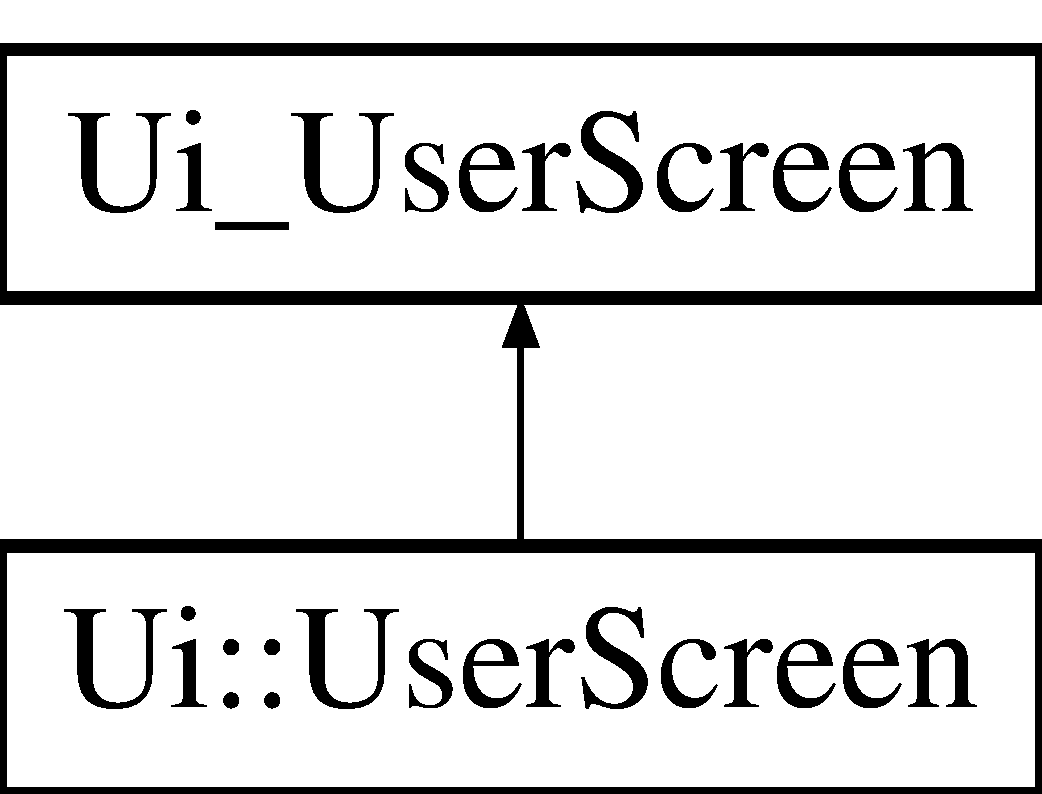
\includegraphics[height=2.000000cm]{classUi__UserScreen}
\end{center}
\end{figure}
\subsection*{Загальнодоступні елементи}
\begin{DoxyCompactItemize}
\item 
\hypertarget{classUi__UserScreen_a54b3d739bdce488848cf19068dfe164e}{void {\bfseries setup\-Ui} (Q\-Main\-Window $\ast$\hyperlink{classUserScreen}{User\-Screen})}\label{classUi__UserScreen_a54b3d739bdce488848cf19068dfe164e}

\item 
\hypertarget{classUi__UserScreen_aeadabe075b2171763d186a2ceaf61314}{void {\bfseries retranslate\-Ui} (Q\-Main\-Window $\ast$\hyperlink{classUserScreen}{User\-Screen})}\label{classUi__UserScreen_aeadabe075b2171763d186a2ceaf61314}

\item 
\hypertarget{classUi__UserScreen_a54b3d739bdce488848cf19068dfe164e}{void {\bfseries setup\-Ui} (Q\-Main\-Window $\ast$\hyperlink{classUserScreen}{User\-Screen})}\label{classUi__UserScreen_a54b3d739bdce488848cf19068dfe164e}

\item 
\hypertarget{classUi__UserScreen_aeadabe075b2171763d186a2ceaf61314}{void {\bfseries retranslate\-Ui} (Q\-Main\-Window $\ast$\hyperlink{classUserScreen}{User\-Screen})}\label{classUi__UserScreen_aeadabe075b2171763d186a2ceaf61314}

\item 
\hypertarget{classUi__UserScreen_a54b3d739bdce488848cf19068dfe164e}{void {\bfseries setup\-Ui} (Q\-Main\-Window $\ast$\hyperlink{classUserScreen}{User\-Screen})}\label{classUi__UserScreen_a54b3d739bdce488848cf19068dfe164e}

\item 
\hypertarget{classUi__UserScreen_aeadabe075b2171763d186a2ceaf61314}{void {\bfseries retranslate\-Ui} (Q\-Main\-Window $\ast$\hyperlink{classUserScreen}{User\-Screen})}\label{classUi__UserScreen_aeadabe075b2171763d186a2ceaf61314}

\end{DoxyCompactItemize}
\subsection*{Загальнодоступні атрибути}
\begin{DoxyCompactItemize}
\item 
\hypertarget{classUi__UserScreen_adc92cff7af8f422e5dcfaa77222cb3f2}{Q\-Widget $\ast$ {\bfseries centralwidget}}\label{classUi__UserScreen_adc92cff7af8f422e5dcfaa77222cb3f2}

\item 
\hypertarget{classUi__UserScreen_a95dc3007529cc02c13c783611d34765b}{Q\-Widget $\ast$ {\bfseries widget}}\label{classUi__UserScreen_a95dc3007529cc02c13c783611d34765b}

\item 
\hypertarget{classUi__UserScreen_ae811c33aa253daf14a377b414b4baca1}{Q\-H\-Box\-Layout $\ast$ {\bfseries horizontal\-Layout\-\_\-4}}\label{classUi__UserScreen_ae811c33aa253daf14a377b414b4baca1}

\item 
\hypertarget{classUi__UserScreen_aab9db9b572882f931025c2fca460c52b}{Q\-V\-Box\-Layout $\ast$ {\bfseries vertical\-Layout}}\label{classUi__UserScreen_aab9db9b572882f931025c2fca460c52b}

\item 
\hypertarget{classUi__UserScreen_ae74ff2cc9500a895a1b24efa1ba10ffe}{Q\-Label $\ast$ {\bfseries label\-\_\-3}}\label{classUi__UserScreen_ae74ff2cc9500a895a1b24efa1ba10ffe}

\item 
\hypertarget{classUi__UserScreen_a58e22c3f9eeeacc28cca723d1c9fc2ee}{Q\-H\-Box\-Layout $\ast$ {\bfseries horizontal\-Layout}}\label{classUi__UserScreen_a58e22c3f9eeeacc28cca723d1c9fc2ee}

\item 
\hypertarget{classUi__UserScreen_a141635bf864747eacafe8667858f2118}{Q\-Spacer\-Item $\ast$ {\bfseries horizontal\-Spacer\-\_\-2}}\label{classUi__UserScreen_a141635bf864747eacafe8667858f2118}

\item 
\hypertarget{classUi__UserScreen_a029f748761908f5e58eb168ccd467fd0}{Q\-Push\-Button $\ast$ {\bfseries push\-Button}}\label{classUi__UserScreen_a029f748761908f5e58eb168ccd467fd0}

\item 
\hypertarget{classUi__UserScreen_a43c2e1e08a93c3dd6a9fa96ec230c993}{Q\-Spacer\-Item $\ast$ {\bfseries horizontal\-Spacer}}\label{classUi__UserScreen_a43c2e1e08a93c3dd6a9fa96ec230c993}

\item 
\hypertarget{classUi__UserScreen_a3cf2e39d787ae79863a7e600398d1186}{Q\-H\-Box\-Layout $\ast$ {\bfseries horizontal\-Layout\-\_\-2}}\label{classUi__UserScreen_a3cf2e39d787ae79863a7e600398d1186}

\item 
\hypertarget{classUi__UserScreen_a4dc94b70e2a6b48902c99f5975e3bea7}{Q\-Label $\ast$ {\bfseries label}}\label{classUi__UserScreen_a4dc94b70e2a6b48902c99f5975e3bea7}

\item 
\hypertarget{classUi__UserScreen_a7a5ef858a41a0ea4327ef295f891a32c}{Q\-Spin\-Box $\ast$ {\bfseries spin\-Box}}\label{classUi__UserScreen_a7a5ef858a41a0ea4327ef295f891a32c}

\item 
\hypertarget{classUi__UserScreen_ab535d42929e47a93c2d9ff787cdcc9fd}{Q\-Label $\ast$ {\bfseries label\-\_\-2}}\label{classUi__UserScreen_ab535d42929e47a93c2d9ff787cdcc9fd}

\item 
\hypertarget{classUi__UserScreen_a6d55991b0fd389c533f71395d622f083}{Q\-H\-Box\-Layout $\ast$ {\bfseries horizontal\-Layout\-\_\-3}}\label{classUi__UserScreen_a6d55991b0fd389c533f71395d622f083}

\item 
\hypertarget{classUi__UserScreen_a44dfb4b5a7ba85003a17ddecb68c5ebf}{Q\-Spacer\-Item $\ast$ {\bfseries horizontal\-Spacer\-\_\-3}}\label{classUi__UserScreen_a44dfb4b5a7ba85003a17ddecb68c5ebf}

\item 
\hypertarget{classUi__UserScreen_a564406d1ccb6bb35ee22d1db6c856290}{Q\-Push\-Button $\ast$ {\bfseries push\-Button\-\_\-2}}\label{classUi__UserScreen_a564406d1ccb6bb35ee22d1db6c856290}

\item 
\hypertarget{classUi__UserScreen_a01543ce099d695124b2bcf37ed63a38f}{Q\-Spacer\-Item $\ast$ {\bfseries horizontal\-Spacer\-\_\-4}}\label{classUi__UserScreen_a01543ce099d695124b2bcf37ed63a38f}

\item 
\hypertarget{classUi__UserScreen_a23acaea5124ffe328316135374034816}{Q\-V\-Box\-Layout $\ast$ {\bfseries vertical\-Layout\-\_\-3}}\label{classUi__UserScreen_a23acaea5124ffe328316135374034816}

\item 
\hypertarget{classUi__UserScreen_ac7c6aec37f22c5081fa40fc82b483a10}{Q\-Label $\ast$ {\bfseries label\-\_\-9}}\label{classUi__UserScreen_ac7c6aec37f22c5081fa40fc82b483a10}

\item 
\hypertarget{classUi__UserScreen_a59af5dacfe2f5372444e7de81f46627f}{Q\-V\-Box\-Layout $\ast$ {\bfseries vertical\-Layout\-\_\-2}}\label{classUi__UserScreen_a59af5dacfe2f5372444e7de81f46627f}

\item 
\hypertarget{classUi__UserScreen_a36c0975e137bf268c08a2012d9a2d24e}{Q\-Combo\-Box $\ast$ {\bfseries combo\-Box}}\label{classUi__UserScreen_a36c0975e137bf268c08a2012d9a2d24e}

\item 
\hypertarget{classUi__UserScreen_a8952446c26e475049af4769c6de41cc6}{Q\-Spacer\-Item $\ast$ {\bfseries vertical\-Spacer}}\label{classUi__UserScreen_a8952446c26e475049af4769c6de41cc6}

\item 
\hypertarget{classUi__UserScreen_ad1e2fc8f7f5c2d7eb8f66f72bc3e626c}{Q\-Push\-Button $\ast$ {\bfseries push\-Button\-\_\-3}}\label{classUi__UserScreen_ad1e2fc8f7f5c2d7eb8f66f72bc3e626c}

\item 
\hypertarget{classUi__UserScreen_a7fa1f4bb475159dea48bdf84ffa2a03d}{Q\-Spacer\-Item $\ast$ {\bfseries vertical\-Spacer\-\_\-2}}\label{classUi__UserScreen_a7fa1f4bb475159dea48bdf84ffa2a03d}

\item 
\hypertarget{classUi__UserScreen_a727ae2b1e909a5249972dbb1e51e2fce}{Q\-Frame $\ast$ {\bfseries line}}\label{classUi__UserScreen_a727ae2b1e909a5249972dbb1e51e2fce}

\item 
\hypertarget{classUi__UserScreen_a500fccaa9d902dfd47a88345169c43f8}{Q\-Label $\ast$ {\bfseries label\-\_\-4}}\label{classUi__UserScreen_a500fccaa9d902dfd47a88345169c43f8}

\item 
\hypertarget{classUi__UserScreen_a357650bb4e513f1808a0f14ecc1f2bc6}{Q\-Grid\-Layout $\ast$ {\bfseries grid\-Layout}}\label{classUi__UserScreen_a357650bb4e513f1808a0f14ecc1f2bc6}

\item 
\hypertarget{classUi__UserScreen_a89d78ff0c89cea37065a0a4c8a8f8e5f}{Q\-Label $\ast$ {\bfseries label\-\_\-5}}\label{classUi__UserScreen_a89d78ff0c89cea37065a0a4c8a8f8e5f}

\item 
\hypertarget{classUi__UserScreen_abfba3562f9d80c2468dfdda67c723259}{Q\-Label $\ast$ {\bfseries label\-\_\-6}}\label{classUi__UserScreen_abfba3562f9d80c2468dfdda67c723259}

\item 
\hypertarget{classUi__UserScreen_a57a36cf6e2388927e7acdaa43ace19b2}{Q\-Slider $\ast$ {\bfseries horizontal\-Slider\-\_\-2}}\label{classUi__UserScreen_a57a36cf6e2388927e7acdaa43ace19b2}

\item 
\hypertarget{classUi__UserScreen_aad1f88c242894492830b58ea3f3d783a}{Q\-Label $\ast$ {\bfseries label\-\_\-7}}\label{classUi__UserScreen_aad1f88c242894492830b58ea3f3d783a}

\item 
\hypertarget{classUi__UserScreen_a2660cf76b6c5d53244b990e0ad76e7f4}{Q\-Label $\ast$ {\bfseries label\-\_\-8}}\label{classUi__UserScreen_a2660cf76b6c5d53244b990e0ad76e7f4}

\item 
\hypertarget{classUi__UserScreen_aa8a10f18cb899db1a6a8b30efd2ecdca}{Q\-Slider $\ast$ {\bfseries horizontal\-Slider\-\_\-4}}\label{classUi__UserScreen_aa8a10f18cb899db1a6a8b30efd2ecdca}

\item 
\hypertarget{classUi__UserScreen_afd05cb4039d10a19d4b33db410a18698}{Q\-Slider $\ast$ {\bfseries horizontal\-Slider}}\label{classUi__UserScreen_afd05cb4039d10a19d4b33db410a18698}

\item 
\hypertarget{classUi__UserScreen_a58ee9b1ba684a8c83c1e1e3e86954cf2}{Q\-Slider $\ast$ {\bfseries horizontal\-Slider\-\_\-3}}\label{classUi__UserScreen_a58ee9b1ba684a8c83c1e1e3e86954cf2}

\item 
\hypertarget{classUi__UserScreen_a93f91b432f75a6cf25fa35e8bb4d64d3}{Q\-Widget $\ast$ {\bfseries layout\-Widget}}\label{classUi__UserScreen_a93f91b432f75a6cf25fa35e8bb4d64d3}

\end{DoxyCompactItemize}


Документація цього класу була створена з файлу\-:\begin{DoxyCompactItemize}
\item 
Recognitor/ui\-\_\-userscreen.\-h\end{DoxyCompactItemize}

\hypertarget{classUserScreen}{\section{Клас User\-Screen}
\label{classUserScreen}\index{User\-Screen@{User\-Screen}}
}
\subsection*{Загальнодоступні елементи}
\begin{DoxyCompactItemize}
\item 
\hypertarget{classUserScreen_a27136456b8f1b4d10dfe1cbfc9c43d7c}{{\bfseries User\-Screen} (Q\-Widget $\ast$parent=0)}\label{classUserScreen_a27136456b8f1b4d10dfe1cbfc9c43d7c}

\end{DoxyCompactItemize}
\subsection*{Приватні слоти}
\begin{DoxyCompactItemize}
\item 
\hypertarget{classUserScreen_a6e25c29ff53726317f4056b66fcb9a18}{void {\bfseries on\-\_\-push\-Button\-\_\-2\-\_\-clicked} ()}\label{classUserScreen_a6e25c29ff53726317f4056b66fcb9a18}

\item 
\hypertarget{classUserScreen_a6e79ba614aa7a1af1520cc78d5e7c264}{void {\bfseries on\-\_\-push\-Button\-\_\-clicked} ()}\label{classUserScreen_a6e79ba614aa7a1af1520cc78d5e7c264}

\end{DoxyCompactItemize}
\subsection*{Приватні дані}
\begin{DoxyCompactItemize}
\item 
\hypertarget{classUserScreen_ade24b1857f428a1a247fd622a51c8de8}{\hyperlink{classUi_1_1UserScreen}{Ui\-::\-User\-Screen} $\ast$ {\bfseries ui}}\label{classUserScreen_ade24b1857f428a1a247fd622a51c8de8}

\end{DoxyCompactItemize}


Документація цих класів була створена з файлів\-:\begin{DoxyCompactItemize}
\item 
Recognitor/\hyperlink{userscreen_8h}{userscreen.\-h}\item 
Recognitor/\hyperlink{userscreen_8cpp}{userscreen.\-cpp}\end{DoxyCompactItemize}

\hypertarget{classUi_1_1UserScreen}{\section{Клас Ui\-:\-:User\-Screen}
\label{classUi_1_1UserScreen}\index{Ui\-::\-User\-Screen@{Ui\-::\-User\-Screen}}
}
Схема успадкувань для Ui\-:\-:User\-Screen\begin{figure}[H]
\begin{center}
\leavevmode
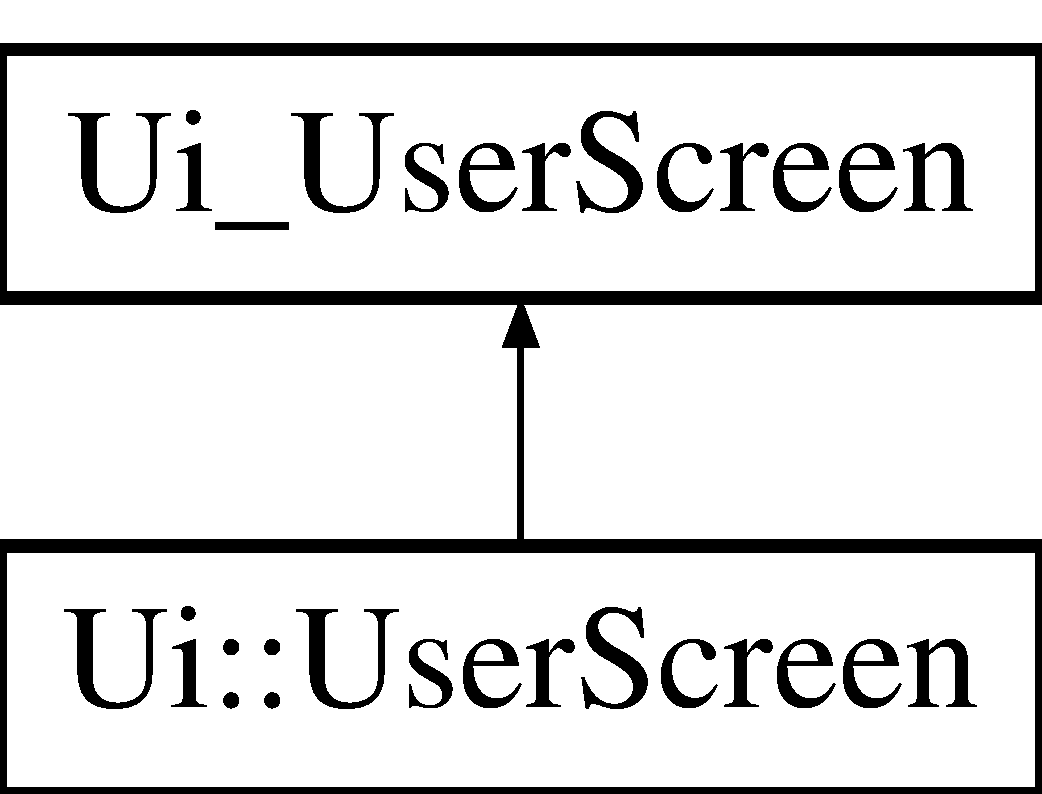
\includegraphics[height=2.000000cm]{classUi_1_1UserScreen}
\end{center}
\end{figure}
\subsection*{Additional Inherited Members}


Документація цього класу була створена з файлу\-:\begin{DoxyCompactItemize}
\item 
Recognitor-\/build-\/desktop-\/\-Qt\-\_\-4\-\_\-8\-\_\-3\-\_\-in\-\_\-\-P\-A\-T\-H\-\_\-\-\_\-\-System\-\_\-\-\_\-\-Release/ui\-\_\-userscreen.\-h\end{DoxyCompactItemize}

\hypertarget{classWindowManager}{\section{Клас Window\-Manager}
\label{classWindowManager}\index{Window\-Manager@{Window\-Manager}}
}


A class for switching between windows of the application.  




{\ttfamily \#include $<$windowmanager.\-h$>$}

\subsection*{Загальнодоступні елементи}
\begin{DoxyCompactItemize}
\item 
\hypertarget{classWindowManager_a3a283b34c19aaa20296befaabad4d29b}{\hyperlink{classWindowManager_a3a283b34c19aaa20296befaabad4d29b}{Window\-Manager} ()}\label{classWindowManager_a3a283b34c19aaa20296befaabad4d29b}

\begin{DoxyCompactList}\small\item\em \hyperlink{classWindowManager}{Window\-Manager} constructor. \end{DoxyCompactList}\item 
void \hyperlink{classWindowManager_a57acbed2b942f979ea6a096cdfca4a3e}{Init} (\hyperlink{classMainWindow}{Main\-Window} $\ast$m, \hyperlink{classAdminScreen}{Admin\-Screen} $\ast$a, \hyperlink{classUserScreen}{User\-Screen} $\ast$u, \hyperlink{classExUserScreen}{Ex\-User\-Screen} $\ast$x, \hyperlink{classGoodsMgmtScreen}{Goods\-Mgmt\-Screen} $\ast$g)
\begin{DoxyCompactList}\small\item\em Initialization function. \end{DoxyCompactList}\end{DoxyCompactItemize}
\subsection*{Загальнодоступні атрибути}
\begin{DoxyCompactItemize}
\item 
\hypertarget{classWindowManager_a9cb795acc230eca8bb2fff11f461fd70}{\hyperlink{classMainWindow}{Main\-Window} $\ast$ \hyperlink{classWindowManager_a9cb795acc230eca8bb2fff11f461fd70}{mw}}\label{classWindowManager_a9cb795acc230eca8bb2fff11f461fd70}

\begin{DoxyCompactList}\small\item\em \hyperlink{classMainWindow}{Main\-Window} reference. \end{DoxyCompactList}\item 
\hypertarget{classWindowManager_ac9607896ec2c594ea376f93a2a8c8e7a}{\hyperlink{classAdminScreen}{Admin\-Screen} $\ast$ \hyperlink{classWindowManager_ac9607896ec2c594ea376f93a2a8c8e7a}{ad}}\label{classWindowManager_ac9607896ec2c594ea376f93a2a8c8e7a}

\begin{DoxyCompactList}\small\item\em \hyperlink{classAdminScreen}{Admin\-Screen} reference. \end{DoxyCompactList}\item 
\hypertarget{classWindowManager_ad6bc24911495de7f8d1e39ae00914475}{\hyperlink{classUserScreen}{User\-Screen} $\ast$ \hyperlink{classWindowManager_ad6bc24911495de7f8d1e39ae00914475}{us}}\label{classWindowManager_ad6bc24911495de7f8d1e39ae00914475}

\begin{DoxyCompactList}\small\item\em \hyperlink{classUserScreen}{User\-Screen} reference. \end{DoxyCompactList}\item 
\hypertarget{classWindowManager_aac54a8f35c47119698b5c52c8d3505b5}{\hyperlink{classExUserScreen}{Ex\-User\-Screen} $\ast$ \hyperlink{classWindowManager_aac54a8f35c47119698b5c52c8d3505b5}{xu}}\label{classWindowManager_aac54a8f35c47119698b5c52c8d3505b5}

\begin{DoxyCompactList}\small\item\em \hyperlink{classExUserScreen}{Ex\-User\-Screen} reference. \end{DoxyCompactList}\item 
\hypertarget{classWindowManager_a5a8f87cbdf8dea57eca5d826de2a1255}{\hyperlink{classGoodsMgmtScreen}{Goods\-Mgmt\-Screen} $\ast$ \hyperlink{classWindowManager_a5a8f87cbdf8dea57eca5d826de2a1255}{gs}}\label{classWindowManager_a5a8f87cbdf8dea57eca5d826de2a1255}

\begin{DoxyCompactList}\small\item\em \hyperlink{classGoodsMgmtScreen}{Goods\-Mgmt\-Screen} reference. \end{DoxyCompactList}\end{DoxyCompactItemize}


\subsection{Детальний опис}
A class for switching between windows of the application. 

\subsection{Опис методів компонент}
\hypertarget{classWindowManager_a57acbed2b942f979ea6a096cdfca4a3e}{\index{Window\-Manager@{Window\-Manager}!Init@{Init}}
\index{Init@{Init}!WindowManager@{Window\-Manager}}
\subsubsection[{Init}]{\setlength{\rightskip}{0pt plus 5cm}void Window\-Manager\-::\-Init (
\begin{DoxyParamCaption}
\item[{{\bf Main\-Window} $\ast$}]{m, }
\item[{{\bf Admin\-Screen} $\ast$}]{a, }
\item[{{\bf User\-Screen} $\ast$}]{u, }
\item[{{\bf Ex\-User\-Screen} $\ast$}]{x, }
\item[{{\bf Goods\-Mgmt\-Screen} $\ast$}]{g}
\end{DoxyParamCaption}
)}}\label{classWindowManager_a57acbed2b942f979ea6a096cdfca4a3e}


Initialization function. 


\begin{DoxyParams}[1]{Аргументи}
\mbox{\tt in}  & {\em m} & -\/ \hyperlink{classMainWindow}{Main\-Window} reference \\
\hline
\mbox{\tt in}  & {\em a} & -\/ \hyperlink{classAdminScreen}{Admin\-Screen} reference \\
\hline
\mbox{\tt in}  & {\em u} & -\/ \hyperlink{classUserScreen}{User\-Screen} reference \\
\hline
\mbox{\tt in}  & {\em x} & -\/ \hyperlink{classExUserScreen}{Ex\-User\-Screen} reference \\
\hline
\mbox{\tt in}  & {\em g} & -\/ \hyperlink{classGoodsMgmtScreen}{Goods\-Mgmt\-Screen} reference \\
\hline
\end{DoxyParams}


Документація цих класів була створена з файлів\-:\begin{DoxyCompactItemize}
\item 
Recognitor/\hyperlink{windowmanager_8h}{windowmanager.\-h}\item 
Recognitor/\hyperlink{windowmanager_8cpp}{windowmanager.\-cpp}\end{DoxyCompactItemize}

\chapter{Файли}
\hypertarget{adminscreen_8cpp}{\section{Файл Recognitor/adminscreen.cpp}
\label{adminscreen_8cpp}\index{Recognitor/adminscreen.\-cpp@{Recognitor/adminscreen.\-cpp}}
}


Administration window implementation.  


{\ttfamily \#include \char`\"{}adminscreen.\-h\char`\"{}}\\*
{\ttfamily \#include \char`\"{}ui\-\_\-adminscreen.\-h\char`\"{}}\\*
{\ttfamily \#include \char`\"{}windowmanager.\-h\char`\"{}}\\*
{\ttfamily \#include $<$Q\-Message\-Box$>$}\\*
\subsection*{Змінні}
\begin{DoxyCompactItemize}
\item 
\hyperlink{classWindowManager}{Window\-Manager} \hyperlink{adminscreen_8cpp_a398def1a3b87c400e0a053b875bf4d93}{W\-Mgr}
\begin{DoxyCompactList}\small\item\em Window Manager instance. \end{DoxyCompactList}\end{DoxyCompactItemize}


\subsection{Детальний опис}
Administration window implementation. \begin{DoxyAuthor}{Автор}
mnxoid
\end{DoxyAuthor}
Copyright 2014 by mnxoid,

This software is the confidential and proprietary information of mnxoid (\char`\"{}\-Confidential Information\char`\"{}). You shall not disclose such Confidential Information and shall use it only in accordance with the terms of the license agreement you entered into with mnxoid. 

\subsection{Опис змінних}
\hypertarget{adminscreen_8cpp_a398def1a3b87c400e0a053b875bf4d93}{\index{adminscreen.\-cpp@{adminscreen.\-cpp}!W\-Mgr@{W\-Mgr}}
\index{W\-Mgr@{W\-Mgr}!adminscreen.cpp@{adminscreen.\-cpp}}
\subsubsection[{W\-Mgr}]{\setlength{\rightskip}{0pt plus 5cm}{\bf Window\-Manager} W\-Mgr}}\label{adminscreen_8cpp_a398def1a3b87c400e0a053b875bf4d93}


Window Manager instance. 

\begin{DoxySeeAlso}{Див. також}
\hyperlink{main_8cpp}{main.\-cpp}
\end{DoxySeeAlso}
Window Manager instance. 
\hypertarget{adminscreen_8h}{\section{Файл Recognitor/adminscreen.h}
\label{adminscreen_8h}\index{Recognitor/adminscreen.\-h@{Recognitor/adminscreen.\-h}}
}


Administration window header.  


{\ttfamily \#include $<$Q\-Main\-Window$>$}\\*
\subsection*{Класи}
\begin{DoxyCompactItemize}
\item 
class \hyperlink{classAdminScreen}{Admin\-Screen}
\end{DoxyCompactItemize}


\subsection{Детальний опис}
Administration window header. \begin{DoxyAuthor}{Автор}
mnxoid
\end{DoxyAuthor}
Copyright 2014 by mnxoid,

This software is the confidential and proprietary information of mnxoid (\char`\"{}\-Confidential Information\char`\"{}). You shall not disclose such Confidential Information and shall use it only in accordance with the terms of the license agreement you entered into with mnxoid. 
\hypertarget{auth_8cpp}{\section{Файл Recognitor/auth.cpp}
\label{auth_8cpp}\index{Recognitor/auth.\-cpp@{Recognitor/auth.\-cpp}}
}


Authentication implementation.  


{\ttfamily \#include \char`\"{}auth.\-h\char`\"{}}\\*
{\ttfamily \#include $<$Q\-String$>$}\\*
{\ttfamily \#include $<$Q\-Debug$>$}\\*
{\ttfamily \#include \char`\"{}packet.\-h\char`\"{}}\\*
\subsection*{Функції}
\begin{DoxyCompactItemize}
\item 
\hyperlink{auth_8h_a7da68dc8ab4fb9bae588bdd1f6afc951}{Access} \hyperlink{auth_8cpp_a4d0f4bb0edb145ecb5a92671df487468}{Check} (Q\-String login, Q\-String pwd)
\begin{DoxyCompactList}\small\item\em The authentication function. \end{DoxyCompactList}\end{DoxyCompactItemize}
\subsection*{Змінні}
\begin{DoxyCompactItemize}
\item 
int \hyperlink{auth_8cpp_aa3399d04c16cf0fde5d6280bd3abd803}{session}
\begin{DoxyCompactList}\small\item\em Current S\-E\-S\-S\-I\-O\-N\-\_\-\-I\-D. \end{DoxyCompactList}\end{DoxyCompactItemize}


\subsection{Детальний опис}
Authentication implementation. \begin{DoxyAuthor}{Автор}
mnxoid
\end{DoxyAuthor}
Copyright 2014 by mnxoid,

This software is the confidential and proprietary information of mnxoid (\char`\"{}\-Confidential Information\char`\"{}). You shall not disclose such Confidential Information and shall use it only in accordance with the terms of the license agreement you entered into with mnxoid. 

\subsection{Опис функцій}
\hypertarget{auth_8cpp_a4d0f4bb0edb145ecb5a92671df487468}{\index{auth.\-cpp@{auth.\-cpp}!Check@{Check}}
\index{Check@{Check}!auth.cpp@{auth.\-cpp}}
\subsubsection[{Check}]{\setlength{\rightskip}{0pt plus 5cm}{\bf Access} Check (
\begin{DoxyParamCaption}
\item[{Q\-String}]{login, }
\item[{Q\-String}]{pwd}
\end{DoxyParamCaption}
)}}\label{auth_8cpp_a4d0f4bb0edb145ecb5a92671df487468}


The authentication function. 


\begin{DoxyParams}[1]{Аргументи}
\mbox{\tt in}  & {\em login} & -\/ User name \\
\hline
\mbox{\tt in}  & {\em pwd} & -\/ User password\\
\hline
\end{DoxyParams}
\begin{DoxyReturn}{Повертає}
Access Privilege level 
\end{DoxyReturn}
\begin{DoxySeeAlso}{Див. також}
\hyperlink{auth_8h_a7da68dc8ab4fb9bae588bdd1f6afc951}{Access} 
\end{DoxySeeAlso}


\subsection{Опис змінних}
\hypertarget{auth_8cpp_aa3399d04c16cf0fde5d6280bd3abd803}{\index{auth.\-cpp@{auth.\-cpp}!session@{session}}
\index{session@{session}!auth.cpp@{auth.\-cpp}}
\subsubsection[{session}]{\setlength{\rightskip}{0pt plus 5cm}int session}}\label{auth_8cpp_aa3399d04c16cf0fde5d6280bd3abd803}


Current S\-E\-S\-S\-I\-O\-N\-\_\-\-I\-D. 

Current S\-E\-S\-S\-I\-O\-N\-\_\-\-I\-D. 
\hypertarget{auth_8h}{\section{Файл Recognitor/auth.h}
\label{auth_8h}\index{Recognitor/auth.\-h@{Recognitor/auth.\-h}}
}


Authentication header.  


\subsection*{Переліки}
\begin{DoxyCompactItemize}
\item 
enum \hyperlink{auth_8h_a7da68dc8ab4fb9bae588bdd1f6afc951}{Access} \{ \hyperlink{auth_8h_a7da68dc8ab4fb9bae588bdd1f6afc951a3228e792244f936584abc6e3d7542d2c}{A\-D\-M\-I\-N}, 
\hyperlink{auth_8h_a7da68dc8ab4fb9bae588bdd1f6afc951a02570c2bd30d794ff48c3b6369fb3545}{E\-X\-U\-S\-E\-R}, 
\hyperlink{auth_8h_a7da68dc8ab4fb9bae588bdd1f6afc951ae2d30a195cee6b2961cc2c23ea4b520b}{U\-S\-E\-R}, 
\hyperlink{auth_8h_a7da68dc8ab4fb9bae588bdd1f6afc951a08f1ea1cb5cac34a4f4237e5259fcabb}{D\-E\-N\-I\-E\-D}
 \}
\begin{DoxyCompactList}\small\item\em Enumeration with types of access privileges. \end{DoxyCompactList}\end{DoxyCompactItemize}
\subsection*{Функції}
\begin{DoxyCompactItemize}
\item 
\hyperlink{auth_8h_a7da68dc8ab4fb9bae588bdd1f6afc951}{Access} \hyperlink{auth_8h_a4d0f4bb0edb145ecb5a92671df487468}{Check} (Q\-String login, Q\-String pwd)
\begin{DoxyCompactList}\small\item\em The authentication function. \end{DoxyCompactList}\end{DoxyCompactItemize}
\subsection*{Змінні}
\begin{DoxyCompactItemize}
\item 
\hypertarget{auth_8h_aa3399d04c16cf0fde5d6280bd3abd803}{int \hyperlink{auth_8h_aa3399d04c16cf0fde5d6280bd3abd803}{session}}\label{auth_8h_aa3399d04c16cf0fde5d6280bd3abd803}

\begin{DoxyCompactList}\small\item\em Current S\-E\-S\-S\-I\-O\-N\-\_\-\-I\-D. \end{DoxyCompactList}\end{DoxyCompactItemize}


\subsection{Детальний опис}
Authentication header. \begin{DoxyAuthor}{Автор}
mnxoid
\end{DoxyAuthor}
Copyright 2014 by mnxoid,

This software is the confidential and proprietary information of mnxoid (\char`\"{}\-Confidential Information\char`\"{}). You shall not disclose such Confidential Information and shall use it only in accordance with the terms of the license agreement you entered into with mnxoid. 

\subsection{Опис переліків}
\hypertarget{auth_8h_a7da68dc8ab4fb9bae588bdd1f6afc951}{\index{auth.\-h@{auth.\-h}!Access@{Access}}
\index{Access@{Access}!auth.h@{auth.\-h}}
\subsubsection[{Access}]{\setlength{\rightskip}{0pt plus 5cm}enum {\bf Access}}}\label{auth_8h_a7da68dc8ab4fb9bae588bdd1f6afc951}


Enumeration with types of access privileges. 

\begin{Desc}
\item[Елементи переліків\-: ]\par
\begin{description}
\index{A\-D\-M\-I\-N@{A\-D\-M\-I\-N}!auth.\-h@{auth.\-h}}\index{auth.\-h@{auth.\-h}!A\-D\-M\-I\-N@{A\-D\-M\-I\-N}}\item[{\em 
\hypertarget{auth_8h_a7da68dc8ab4fb9bae588bdd1f6afc951a3228e792244f936584abc6e3d7542d2c}{A\-D\-M\-I\-N}\label{auth_8h_a7da68dc8ab4fb9bae588bdd1f6afc951a3228e792244f936584abc6e3d7542d2c}
}]Administrator privileges. \index{E\-X\-U\-S\-E\-R@{E\-X\-U\-S\-E\-R}!auth.\-h@{auth.\-h}}\index{auth.\-h@{auth.\-h}!E\-X\-U\-S\-E\-R@{E\-X\-U\-S\-E\-R}}\item[{\em 
\hypertarget{auth_8h_a7da68dc8ab4fb9bae588bdd1f6afc951a02570c2bd30d794ff48c3b6369fb3545}{E\-X\-U\-S\-E\-R}\label{auth_8h_a7da68dc8ab4fb9bae588bdd1f6afc951a02570c2bd30d794ff48c3b6369fb3545}
}]Extended user privileges. \index{U\-S\-E\-R@{U\-S\-E\-R}!auth.\-h@{auth.\-h}}\index{auth.\-h@{auth.\-h}!U\-S\-E\-R@{U\-S\-E\-R}}\item[{\em 
\hypertarget{auth_8h_a7da68dc8ab4fb9bae588bdd1f6afc951ae2d30a195cee6b2961cc2c23ea4b520b}{U\-S\-E\-R}\label{auth_8h_a7da68dc8ab4fb9bae588bdd1f6afc951ae2d30a195cee6b2961cc2c23ea4b520b}
}]Default user privileges. \index{D\-E\-N\-I\-E\-D@{D\-E\-N\-I\-E\-D}!auth.\-h@{auth.\-h}}\index{auth.\-h@{auth.\-h}!D\-E\-N\-I\-E\-D@{D\-E\-N\-I\-E\-D}}\item[{\em 
\hypertarget{auth_8h_a7da68dc8ab4fb9bae588bdd1f6afc951a08f1ea1cb5cac34a4f4237e5259fcabb}{D\-E\-N\-I\-E\-D}\label{auth_8h_a7da68dc8ab4fb9bae588bdd1f6afc951a08f1ea1cb5cac34a4f4237e5259fcabb}
}]Access denied. \end{description}
\end{Desc}



\subsection{Опис функцій}
\hypertarget{auth_8h_a4d0f4bb0edb145ecb5a92671df487468}{\index{auth.\-h@{auth.\-h}!Check@{Check}}
\index{Check@{Check}!auth.h@{auth.\-h}}
\subsubsection[{Check}]{\setlength{\rightskip}{0pt plus 5cm}{\bf Access} Check (
\begin{DoxyParamCaption}
\item[{Q\-String}]{login, }
\item[{Q\-String}]{pwd}
\end{DoxyParamCaption}
)}}\label{auth_8h_a4d0f4bb0edb145ecb5a92671df487468}


The authentication function. 


\begin{DoxyParams}[1]{Аргументи}
\mbox{\tt in}  & {\em login} & -\/ User name \\
\hline
\mbox{\tt in}  & {\em pwd} & -\/ User password\\
\hline
\end{DoxyParams}
\begin{DoxyReturn}{Повертає}
Access Privilege level 
\end{DoxyReturn}
\begin{DoxySeeAlso}{Див. також}
\hyperlink{auth_8h_a7da68dc8ab4fb9bae588bdd1f6afc951}{Access} 
\end{DoxySeeAlso}

\hypertarget{cameracapture_8cpp}{\section{Файл Recognitor/cameracapture.cpp}
\label{cameracapture_8cpp}\index{Recognitor/cameracapture.\-cpp@{Recognitor/cameracapture.\-cpp}}
}


Camera capturing class implementation.  


{\ttfamily \#include \char`\"{}cameracapture.\-h\char`\"{}}\\*
{\ttfamily \#include $<$opencv2/highgui/highgui.\-hpp$>$}\\*
{\ttfamily \#include $<$pthread.\-h$>$}\\*
{\ttfamily \#include $<$Q\-Message\-Box$>$}\\*
{\ttfamily \#include $<$Q\-Debug$>$}\\*


\subsection{Детальний опис}
Camera capturing class implementation. \begin{DoxyAuthor}{Автор}
mnxoid
\end{DoxyAuthor}
Copyright 2014 by mnxoid,

This software is the confidential and proprietary information of mnxoid (\char`\"{}\-Confidential Information\char`\"{}). You shall not disclose such Confidential Information and shall use it only in accordance with the terms of the license agreement you entered into with mnxoid. 
\hypertarget{cameracapture_8h}{\section{Файл Recognitor/cameracapture.h}
\label{cameracapture_8h}\index{Recognitor/cameracapture.\-h@{Recognitor/cameracapture.\-h}}
}


Camera capturing class header.  


{\ttfamily \#include $<$pthread.\-h$>$}\\*
{\ttfamily \#include $<$opencv2/highgui/highgui.\-hpp$>$}\\*
{\ttfamily \#include $<$Q\-Widget$>$}\\*
{\ttfamily \#include $<$Q\-Object$>$}\\*
{\ttfamily \#include $<$Q\-Thread$>$}\\*
\subsection*{Класи}
\begin{DoxyCompactItemize}
\item 
struct \hyperlink{structARGS}{A\-R\-G\-S}
\begin{DoxyCompactList}\small\item\em The arguments for the capturing thread function. \end{DoxyCompactList}\item 
class \hyperlink{classCameraCapture}{Camera\-Capture}
\begin{DoxyCompactList}\small\item\em A class for capturing frames from the camera. \end{DoxyCompactList}\end{DoxyCompactItemize}


\subsection{Детальний опис}
Camera capturing class header. \begin{DoxyAuthor}{Автор}
mnxoid
\end{DoxyAuthor}
Copyright 2014 by mnxoid,

This software is the confidential and proprietary information of mnxoid (\char`\"{}\-Confidential Information\char`\"{}). You shall not disclose such Confidential Information and shall use it only in accordance with the terms of the license agreement you entered into with mnxoid. 
\hypertarget{cvtoqt_8cpp}{\section{Файл Recognitor/cvtoqt.cpp}
\label{cvtoqt_8cpp}\index{Recognitor/cvtoqt.\-cpp@{Recognitor/cvtoqt.\-cpp}}
}


Open\-C\-V-\/\-Qt conversion implementation.  


{\ttfamily \#include $<$Q\-Debug$>$}\\*
{\ttfamily \#include $<$opencv2/highgui/highgui.\-hpp$>$}\\*
{\ttfamily \#include $<$Q\-Image$>$}\\*
{\ttfamily \#include $<$Q\-Rgb$>$}\\*
\subsection*{Функції}
\begin{DoxyCompactItemize}
\item 
Q\-Image \hyperlink{cvtoqt_8cpp_ae59774d7a465e8417e39093b0f52ef98}{Mat\-To\-Q\-Image} (const cv\-::\-Mat \&mat)
\begin{DoxyCompactList}\small\item\em This function converts cv\-::\-Mat to Q\-Image. \end{DoxyCompactList}\end{DoxyCompactItemize}


\subsection{Детальний опис}
Open\-C\-V-\/\-Qt conversion implementation. \begin{DoxyAuthor}{Автор}
mnxoid
\end{DoxyAuthor}
Copyright 2014 by mnxoid,

This software is the confidential and proprietary information of mnxoid (\char`\"{}\-Confidential Information\char`\"{}). You shall not disclose such Confidential Information and shall use it only in accordance with the terms of the license agreement you entered into with mnxoid. 

\subsection{Опис функцій}
\hypertarget{cvtoqt_8cpp_ae59774d7a465e8417e39093b0f52ef98}{\index{cvtoqt.\-cpp@{cvtoqt.\-cpp}!Mat\-To\-Q\-Image@{Mat\-To\-Q\-Image}}
\index{Mat\-To\-Q\-Image@{Mat\-To\-Q\-Image}!cvtoqt.cpp@{cvtoqt.\-cpp}}
\subsubsection[{Mat\-To\-Q\-Image}]{\setlength{\rightskip}{0pt plus 5cm}Q\-Image Mat\-To\-Q\-Image (
\begin{DoxyParamCaption}
\item[{const cv\-::\-Mat \&}]{mat}
\end{DoxyParamCaption}
)}}\label{cvtoqt_8cpp_ae59774d7a465e8417e39093b0f52ef98}


This function converts cv\-::\-Mat to Q\-Image. 


\begin{DoxyParams}[1]{Аргументи}
\mbox{\tt in}  & {\em cv\-::\-Mat\&} & mat -\/ reference to the cv\-::\-Mat to convert\\
\hline
\end{DoxyParams}
\begin{DoxyReturn}{Повертає}
Q\-Image Converted from cv\-::\-Mat 
\end{DoxyReturn}

\hypertarget{cvtoqt_8h}{\section{Файл Recognitor/cvtoqt.h}
\label{cvtoqt_8h}\index{Recognitor/cvtoqt.\-h@{Recognitor/cvtoqt.\-h}}
}


Open\-C\-V-\/\-Qt conversion header.  


{\ttfamily \#include $<$opencv2/highgui/highgui.\-hpp$>$}\\*
\subsection*{Функції}
\begin{DoxyCompactItemize}
\item 
Q\-Image \hyperlink{cvtoqt_8h_ae59774d7a465e8417e39093b0f52ef98}{Mat\-To\-Q\-Image} (const cv\-::\-Mat \&mat)
\begin{DoxyCompactList}\small\item\em This function converts cv\-::\-Mat to Q\-Image. \end{DoxyCompactList}\end{DoxyCompactItemize}


\subsection{Детальний опис}
Open\-C\-V-\/\-Qt conversion header. \begin{DoxyAuthor}{Автор}
mnxoid
\end{DoxyAuthor}
Copyright 2014 by mnxoid,

This software is the confidential and proprietary information of mnxoid (\char`\"{}\-Confidential Information\char`\"{}). You shall not disclose such Confidential Information and shall use it only in accordance with the terms of the license agreement you entered into with mnxoid. 

\subsection{Опис функцій}
\hypertarget{cvtoqt_8h_ae59774d7a465e8417e39093b0f52ef98}{\index{cvtoqt.\-h@{cvtoqt.\-h}!Mat\-To\-Q\-Image@{Mat\-To\-Q\-Image}}
\index{Mat\-To\-Q\-Image@{Mat\-To\-Q\-Image}!cvtoqt.h@{cvtoqt.\-h}}
\subsubsection[{Mat\-To\-Q\-Image}]{\setlength{\rightskip}{0pt plus 5cm}Q\-Image Mat\-To\-Q\-Image (
\begin{DoxyParamCaption}
\item[{const cv\-::\-Mat \&}]{mat}
\end{DoxyParamCaption}
)}}\label{cvtoqt_8h_ae59774d7a465e8417e39093b0f52ef98}


This function converts cv\-::\-Mat to Q\-Image. 


\begin{DoxyParams}[1]{Аргументи}
\mbox{\tt in}  & {\em mat} & -\/ reference to the cv\-::\-Mat to convert\\
\hline
\end{DoxyParams}
\begin{DoxyReturn}{Повертає}
Q\-Image Converted from cv\-::\-Mat
\end{DoxyReturn}

\begin{DoxyParams}[1]{Аргументи}
\mbox{\tt in}  & {\em cv\-::\-Mat\&} & mat -\/ reference to the cv\-::\-Mat to convert\\
\hline
\end{DoxyParams}
\begin{DoxyReturn}{Повертає}
Q\-Image Converted from cv\-::\-Mat 
\end{DoxyReturn}

\hypertarget{exuserscreen_8cpp}{\section{Файл Recognitor/exuserscreen.cpp}
\label{exuserscreen_8cpp}\index{Recognitor/exuserscreen.\-cpp@{Recognitor/exuserscreen.\-cpp}}
}


Extended User window implementation.  


{\ttfamily \#include \char`\"{}exuserscreen.\-h\char`\"{}}\\*
{\ttfamily \#include \char`\"{}ui\-\_\-exuserscreen.\-h\char`\"{}}\\*
{\ttfamily \#include \char`\"{}windowmanager.\-h\char`\"{}}\\*
{\ttfamily \#include $<$Q\-Message\-Box$>$}\\*
{\ttfamily \#include \char`\"{}cameracapture.\-h\char`\"{}}\\*
{\ttfamily \#include \char`\"{}cvtoqt.\-h\char`\"{}}\\*
{\ttfamily \#include $<$Q\-Debug$>$}\\*
\subsection*{Змінні}
\begin{DoxyCompactItemize}
\item 
\hypertarget{exuserscreen_8cpp_add53acba88e1ae4f2143baff6786f953}{int \hyperlink{exuserscreen_8cpp_add53acba88e1ae4f2143baff6786f953}{is\-Capturing} = 0}\label{exuserscreen_8cpp_add53acba88e1ae4f2143baff6786f953}

\begin{DoxyCompactList}\small\item\em Determines, whether capturing session is active. \end{DoxyCompactList}\item 
\hyperlink{classWindowManager}{Window\-Manager} \hyperlink{exuserscreen_8cpp_a398def1a3b87c400e0a053b875bf4d93}{W\-Mgr}
\begin{DoxyCompactList}\small\item\em Window Manager instance. \end{DoxyCompactList}\item 
\hyperlink{classCameraCapture}{Camera\-Capture} $\ast$ \hyperlink{exuserscreen_8cpp_a55ac8a828f46a342155dc9da52187524}{cc}
\begin{DoxyCompactList}\small\item\em Camera capture instance. \end{DoxyCompactList}\end{DoxyCompactItemize}


\subsection{Детальний опис}
Extended User window implementation. \begin{DoxyAuthor}{Автор}
mnxoid
\end{DoxyAuthor}
Copyright 2014 by mnxoid,

This software is the confidential and proprietary information of mnxoid (\char`\"{}\-Confidential Information\char`\"{}). You shall not disclose such Confidential Information and shall use it only in accordance with the terms of the license agreement you entered into with mnxoid. 

\subsection{Опис змінних}
\hypertarget{exuserscreen_8cpp_a55ac8a828f46a342155dc9da52187524}{\index{exuserscreen.\-cpp@{exuserscreen.\-cpp}!cc@{cc}}
\index{cc@{cc}!exuserscreen.cpp@{exuserscreen.\-cpp}}
\subsubsection[{cc}]{\setlength{\rightskip}{0pt plus 5cm}{\bf Camera\-Capture}$\ast$ cc}}\label{exuserscreen_8cpp_a55ac8a828f46a342155dc9da52187524}


Camera capture instance. 

\begin{DoxySeeAlso}{Див. також}
\hyperlink{classCameraCapture}{Camera\-Capture} 
\end{DoxySeeAlso}
\hypertarget{exuserscreen_8cpp_a398def1a3b87c400e0a053b875bf4d93}{\index{exuserscreen.\-cpp@{exuserscreen.\-cpp}!W\-Mgr@{W\-Mgr}}
\index{W\-Mgr@{W\-Mgr}!exuserscreen.cpp@{exuserscreen.\-cpp}}
\subsubsection[{W\-Mgr}]{\setlength{\rightskip}{0pt plus 5cm}{\bf Window\-Manager} W\-Mgr}}\label{exuserscreen_8cpp_a398def1a3b87c400e0a053b875bf4d93}


Window Manager instance. 

\begin{DoxySeeAlso}{Див. також}
\hyperlink{main_8cpp}{main.\-cpp} 
\end{DoxySeeAlso}

\hypertarget{exuserscreen_8h}{\section{Файл Recognitor/exuserscreen.h}
\label{exuserscreen_8h}\index{Recognitor/exuserscreen.\-h@{Recognitor/exuserscreen.\-h}}
}


Extended User window header.  


{\ttfamily \#include $<$Q\-Main\-Window$>$}\\*
{\ttfamily \#include \char`\"{}responsive.\-h\char`\"{}}\\*
{\ttfamily \#include \char`\"{}imshowable.\-h\char`\"{}}\\*
\subsection*{Класи}
\begin{DoxyCompactItemize}
\item 
class \hyperlink{classExUserScreen}{Ex\-User\-Screen}
\begin{DoxyCompactList}\small\item\em Extended User window class. \end{DoxyCompactList}\end{DoxyCompactItemize}
\subsection*{Змінні}
\begin{DoxyCompactItemize}
\item 
\hypertarget{exuserscreen_8h_add53acba88e1ae4f2143baff6786f953}{int \hyperlink{exuserscreen_8h_add53acba88e1ae4f2143baff6786f953}{is\-Capturing}}\label{exuserscreen_8h_add53acba88e1ae4f2143baff6786f953}

\begin{DoxyCompactList}\small\item\em Determines, whether capturing session is active. \end{DoxyCompactList}\end{DoxyCompactItemize}


\subsection{Детальний опис}
Extended User window header. \begin{DoxyAuthor}{Автор}
mnxoid
\end{DoxyAuthor}
Copyright 2014 by mnxoid,

This software is the confidential and proprietary information of mnxoid (\char`\"{}\-Confidential Information\char`\"{}). You shall not disclose such Confidential Information and shall use it only in accordance with the terms of the license agreement you entered into with mnxoid. 
\hypertarget{goodsmgmtscreen_8cpp}{\section{Файл Recognitor/goodsmgmtscreen.cpp}
\label{goodsmgmtscreen_8cpp}\index{Recognitor/goodsmgmtscreen.\-cpp@{Recognitor/goodsmgmtscreen.\-cpp}}
}


Goods management window implementation.  


{\ttfamily \#include \char`\"{}goodsmgmtscreen.\-h\char`\"{}}\\*
{\ttfamily \#include \char`\"{}ui\-\_\-goodsmgmtscreen.\-h\char`\"{}}\\*
{\ttfamily \#include \char`\"{}windowmanager.\-h\char`\"{}}\\*
{\ttfamily \#include $<$Q\-Message\-Box$>$}\\*
\subsection*{Змінні}
\begin{DoxyCompactItemize}
\item 
\hyperlink{classWindowManager}{Window\-Manager} \hyperlink{goodsmgmtscreen_8cpp_a398def1a3b87c400e0a053b875bf4d93}{W\-Mgr}
\begin{DoxyCompactList}\small\item\em \hyperlink{classWindowManager}{Window\-Manager} instance. \end{DoxyCompactList}\end{DoxyCompactItemize}


\subsection{Детальний опис}
Goods management window implementation. \begin{DoxyAuthor}{Автор}
mnxoid
\end{DoxyAuthor}
Copyright 2014 by mnxoid,

This software is the confidential and proprietary information of mnxoid (\char`\"{}\-Confidential Information\char`\"{}). You shall not disclose such Confidential Information and shall use it only in accordance with the terms of the license agreement you entered into with mnxoid. 

\subsection{Опис змінних}
\hypertarget{goodsmgmtscreen_8cpp_a398def1a3b87c400e0a053b875bf4d93}{\index{goodsmgmtscreen.\-cpp@{goodsmgmtscreen.\-cpp}!W\-Mgr@{W\-Mgr}}
\index{W\-Mgr@{W\-Mgr}!goodsmgmtscreen.cpp@{goodsmgmtscreen.\-cpp}}
\subsubsection[{W\-Mgr}]{\setlength{\rightskip}{0pt plus 5cm}{\bf Window\-Manager} W\-Mgr}}\label{goodsmgmtscreen_8cpp_a398def1a3b87c400e0a053b875bf4d93}


\hyperlink{classWindowManager}{Window\-Manager} instance. 

Window Manager instance. 
\hypertarget{goodsmgmtscreen_8h}{\section{Файл Recognitor/goodsmgmtscreen.h}
\label{goodsmgmtscreen_8h}\index{Recognitor/goodsmgmtscreen.\-h@{Recognitor/goodsmgmtscreen.\-h}}
}


Goods management window header.  


{\ttfamily \#include $<$Q\-Main\-Window$>$}\\*
\subsection*{Класи}
\begin{DoxyCompactItemize}
\item 
class \hyperlink{classGoodsMgmtScreen}{Goods\-Mgmt\-Screen}
\end{DoxyCompactItemize}


\subsection{Детальний опис}
Goods management window header. \begin{DoxyAuthor}{Автор}
mnxoid
\end{DoxyAuthor}
Copyright 2014 by mnxoid,

This software is the confidential and proprietary information of mnxoid (\char`\"{}\-Confidential Information\char`\"{}). You shall not disclose such Confidential Information and shall use it only in accordance with the terms of the license agreement you entered into with mnxoid. 
\hypertarget{main_8cpp}{\section{Файл Recognitor/main.cpp}
\label{main_8cpp}\index{Recognitor/main.\-cpp@{Recognitor/main.\-cpp}}
}


Main source file.  


{\ttfamily \#include $<$Q\-Application$>$}\\*
{\ttfamily \#include \char`\"{}mainwindow.\-h\char`\"{}}\\*
{\ttfamily \#include \char`\"{}windowmanager.\-h\char`\"{}}\\*
{\ttfamily \#include $<$X11/\-Xlib.\-h$>$}\\*
{\ttfamily \#include \char`\"{}cameracapture.\-h\char`\"{}}\\*
\subsection*{Функції}
\begin{DoxyCompactItemize}
\item 
\hypertarget{main_8cpp_a0ddf1224851353fc92bfbff6f499fa97}{int {\bfseries main} (int argc, char $\ast$argv\mbox{[}$\,$\mbox{]})}\label{main_8cpp_a0ddf1224851353fc92bfbff6f499fa97}

\end{DoxyCompactItemize}
\subsection*{Змінні}
\begin{DoxyCompactItemize}
\item 
\hyperlink{classWindowManager}{Window\-Manager} \hyperlink{main_8cpp_a398def1a3b87c400e0a053b875bf4d93}{W\-Mgr}
\begin{DoxyCompactList}\small\item\em \hyperlink{classWindowManager}{Window\-Manager} instance. \end{DoxyCompactList}\item 
\hypertarget{main_8cpp_add53acba88e1ae4f2143baff6786f953}{int \hyperlink{main_8cpp_add53acba88e1ae4f2143baff6786f953}{is\-Capturing} = 0}\label{main_8cpp_add53acba88e1ae4f2143baff6786f953}

\begin{DoxyCompactList}\small\item\em Determines, whether capturing session is active. \end{DoxyCompactList}\item 
\hyperlink{classCameraCapture}{Camera\-Capture} $\ast$ \hyperlink{main_8cpp_a55ac8a828f46a342155dc9da52187524}{cc}
\begin{DoxyCompactList}\small\item\em \hyperlink{classCameraCapture}{Camera\-Capture} instance. \end{DoxyCompactList}\end{DoxyCompactItemize}


\subsection{Детальний опис}
Main source file. \begin{DoxyAuthor}{Автор}
mnxoid
\end{DoxyAuthor}
Copyright 2014 by mnxoid,

This software is the confidential and proprietary information of mnxoid (\char`\"{}\-Confidential Information\char`\"{}). You shall not disclose such Confidential Information and shall use it only in accordance with the terms of the license agreement you entered into with mnxoid. 

\subsection{Опис змінних}
\hypertarget{main_8cpp_a55ac8a828f46a342155dc9da52187524}{\index{main.\-cpp@{main.\-cpp}!cc@{cc}}
\index{cc@{cc}!main.cpp@{main.\-cpp}}
\subsubsection[{cc}]{\setlength{\rightskip}{0pt plus 5cm}{\bf Camera\-Capture}$\ast$ cc}}\label{main_8cpp_a55ac8a828f46a342155dc9da52187524}


\hyperlink{classCameraCapture}{Camera\-Capture} instance. 

Camera capture instance. \hypertarget{main_8cpp_a398def1a3b87c400e0a053b875bf4d93}{\index{main.\-cpp@{main.\-cpp}!W\-Mgr@{W\-Mgr}}
\index{W\-Mgr@{W\-Mgr}!main.cpp@{main.\-cpp}}
\subsubsection[{W\-Mgr}]{\setlength{\rightskip}{0pt plus 5cm}{\bf Window\-Manager} W\-Mgr}}\label{main_8cpp_a398def1a3b87c400e0a053b875bf4d93}


\hyperlink{classWindowManager}{Window\-Manager} instance. 

Window Manager instance. 
\hypertarget{mainwindow_8cpp}{\section{Файл Recognitor/mainwindow.cpp}
\label{mainwindow_8cpp}\index{Recognitor/mainwindow.\-cpp@{Recognitor/mainwindow.\-cpp}}
}


Authorization window source.  


{\ttfamily \#include \char`\"{}mainwindow.\-h\char`\"{}}\\*
{\ttfamily \#include \char`\"{}ui\-\_\-mainwindow.\-h\char`\"{}}\\*
{\ttfamily \#include \char`\"{}auth.\-h\char`\"{}}\\*
{\ttfamily \#include \char`\"{}windowmanager.\-h\char`\"{}}\\*
{\ttfamily \#include $<$Q\-Message\-Box$>$}\\*
{\ttfamily \#include \char`\"{}keyenterreceiver.\-h\char`\"{}}\\*
\subsection*{Змінні}
\begin{DoxyCompactItemize}
\item 
\hypertarget{mainwindow_8cpp_ae8d285b499ca83732d68670b69aa53fb}{\hyperlink{classkeyEnterReceiver}{key\-Enter\-Receiver} $\ast$ \hyperlink{mainwindow_8cpp_ae8d285b499ca83732d68670b69aa53fb}{key}}\label{mainwindow_8cpp_ae8d285b499ca83732d68670b69aa53fb}

\begin{DoxyCompactList}\small\item\em Enter key receiver (extracted for the sake of memory management) \end{DoxyCompactList}\item 
\hyperlink{classWindowManager}{Window\-Manager} \hyperlink{mainwindow_8cpp_a398def1a3b87c400e0a053b875bf4d93}{W\-Mgr}
\begin{DoxyCompactList}\small\item\em Window Manager instance. \end{DoxyCompactList}\end{DoxyCompactItemize}


\subsection{Детальний опис}
Authorization window source. \begin{DoxyAuthor}{Автор}
mnxoid
\end{DoxyAuthor}
Copyright 2014 by mnxoid,

This software is the confidential and proprietary information of mnxoid (\char`\"{}\-Confidential Information\char`\"{}). You shall not disclose such Confidential Information and shall use it only in accordance with the terms of the license agreement you entered into with mnxoid. 

\subsection{Опис змінних}
\hypertarget{mainwindow_8cpp_a398def1a3b87c400e0a053b875bf4d93}{\index{mainwindow.\-cpp@{mainwindow.\-cpp}!W\-Mgr@{W\-Mgr}}
\index{W\-Mgr@{W\-Mgr}!mainwindow.cpp@{mainwindow.\-cpp}}
\subsubsection[{W\-Mgr}]{\setlength{\rightskip}{0pt plus 5cm}{\bf Window\-Manager} W\-Mgr}}\label{mainwindow_8cpp_a398def1a3b87c400e0a053b875bf4d93}


Window Manager instance. 

\begin{DoxySeeAlso}{Див. також}
\hyperlink{main_8cpp}{main.\-cpp}
\end{DoxySeeAlso}
Window Manager instance. 
\hypertarget{mainwindow_8h}{\section{Файл Recognitor/mainwindow.h}
\label{mainwindow_8h}\index{Recognitor/mainwindow.\-h@{Recognitor/mainwindow.\-h}}
}


Authorization window header (auto generated)  


{\ttfamily \#include $<$Q\-Main\-Window$>$}\\*
\subsection*{Класи}
\begin{DoxyCompactItemize}
\item 
class \hyperlink{classMainWindow}{Main\-Window}
\end{DoxyCompactItemize}


\subsection{Детальний опис}
Authorization window header (auto generated) \begin{DoxyAuthor}{Автор}
mnxoid
\end{DoxyAuthor}
Copyright 2014 by mnxoid,

This software is the confidential and proprietary information of mnxoid (\char`\"{}\-Confidential Information\char`\"{}). You shall not disclose such Confidential Information and shall use it only in accordance with the terms of the license agreement you entered into with mnxoid. 
\hypertarget{packet_8cpp}{\section{Файл Recognitor/packet.cpp}
\label{packet_8cpp}\index{Recognitor/packet.\-cpp@{Recognitor/packet.\-cpp}}
}


\hyperlink{classPacket}{Packet} class implementation.  


{\ttfamily \#include \char`\"{}packet.\-h\char`\"{}}\\*
{\ttfamily \#include $<$Q\-Tcp\-Socket$>$}\\*
{\ttfamily \#include $<$Q\-I\-O\-Device$>$}\\*


\subsection{Детальний опис}
\hyperlink{classPacket}{Packet} class implementation. \begin{DoxyAuthor}{Автор}
mnxoid
\end{DoxyAuthor}
Copyright 2014 by mnxoid,

This software is the confidential and proprietary information of mnxoid (\char`\"{}\-Confidential Information\char`\"{}). You shall not disclose such Confidential Information and shall use it only in accordance with the terms of the license agreement you entered into with mnxoid. 
\hypertarget{packet_8h}{\section{Файл Recognitor/packet.h}
\label{packet_8h}\index{Recognitor/packet.\-h@{Recognitor/packet.\-h}}
}


\hyperlink{classPacket}{Packet} class header.  


{\ttfamily \#include $<$Q\-Byte\-Array$>$}\\*
{\ttfamily \#include $<$Q\-Tcp\-Server$>$}\\*
\subsection*{Класи}
\begin{DoxyCompactItemize}
\item 
class \hyperlink{classPacket}{Packet}
\begin{DoxyCompactList}\small\item\em A class for Client-\/\-Server communication. \end{DoxyCompactList}\end{DoxyCompactItemize}
\subsection*{Переліки}
\begin{DoxyCompactItemize}
\item 
enum \hyperlink{packet_8h_a15e96d9e79cfa4c3aaba6861be4707e3}{R\-Q\-T\-Y\-P\-E} \{ \hyperlink{packet_8h_a15e96d9e79cfa4c3aaba6861be4707e3a8b22fbb60fcbd7a4a5e1e6ff6ee38218}{A\-U\-T\-H}, 
\hyperlink{packet_8h_a15e96d9e79cfa4c3aaba6861be4707e3a8f3bdca6f4cd81fa46a4e0adfbf14445}{R\-E\-S\-P\-\_\-\-O\-K}, 
\hyperlink{packet_8h_a15e96d9e79cfa4c3aaba6861be4707e3aa442e1876eb255ac7668208ef4678b7e}{R\-E\-S\-P\-\_\-\-E\-R\-R}, 
\hyperlink{packet_8h_a15e96d9e79cfa4c3aaba6861be4707e3a2f0d18fc0d0fa4a6cd92dc328501874d}{E\-M\-P\-T\-Y}
 \}
\begin{DoxyCompactList}\small\item\em Enumeration with types of requests. \end{DoxyCompactList}\end{DoxyCompactItemize}


\subsection{Детальний опис}
\hyperlink{classPacket}{Packet} class header. \begin{DoxyAuthor}{Автор}
mnxoid
\end{DoxyAuthor}
Copyright 2014 by mnxoid,

This software is the confidential and proprietary information of mnxoid (\char`\"{}\-Confidential Information\char`\"{}). You shall not disclose such Confidential Information and shall use it only in accordance with the terms of the license agreement you entered into with mnxoid. 

\subsection{Опис переліків}
\hypertarget{packet_8h_a15e96d9e79cfa4c3aaba6861be4707e3}{\index{packet.\-h@{packet.\-h}!R\-Q\-T\-Y\-P\-E@{R\-Q\-T\-Y\-P\-E}}
\index{R\-Q\-T\-Y\-P\-E@{R\-Q\-T\-Y\-P\-E}!packet.h@{packet.\-h}}
\subsubsection[{R\-Q\-T\-Y\-P\-E}]{\setlength{\rightskip}{0pt plus 5cm}enum {\bf R\-Q\-T\-Y\-P\-E}}}\label{packet_8h_a15e96d9e79cfa4c3aaba6861be4707e3}


Enumeration with types of requests. 

\begin{Desc}
\item[Елементи переліків\-: ]\par
\begin{description}
\index{A\-U\-T\-H@{A\-U\-T\-H}!packet.\-h@{packet.\-h}}\index{packet.\-h@{packet.\-h}!A\-U\-T\-H@{A\-U\-T\-H}}\item[{\em 
\hypertarget{packet_8h_a15e96d9e79cfa4c3aaba6861be4707e3a8b22fbb60fcbd7a4a5e1e6ff6ee38218}{A\-U\-T\-H}\label{packet_8h_a15e96d9e79cfa4c3aaba6861be4707e3a8b22fbb60fcbd7a4a5e1e6ff6ee38218}
}]Authentication. \index{R\-E\-S\-P\-\_\-\-O\-K@{R\-E\-S\-P\-\_\-\-O\-K}!packet.\-h@{packet.\-h}}\index{packet.\-h@{packet.\-h}!R\-E\-S\-P\-\_\-\-O\-K@{R\-E\-S\-P\-\_\-\-O\-K}}\item[{\em 
\hypertarget{packet_8h_a15e96d9e79cfa4c3aaba6861be4707e3a8f3bdca6f4cd81fa46a4e0adfbf14445}{R\-E\-S\-P\-\_\-\-O\-K}\label{packet_8h_a15e96d9e79cfa4c3aaba6861be4707e3a8f3bdca6f4cd81fa46a4e0adfbf14445}
}]Good server response. \index{R\-E\-S\-P\-\_\-\-E\-R\-R@{R\-E\-S\-P\-\_\-\-E\-R\-R}!packet.\-h@{packet.\-h}}\index{packet.\-h@{packet.\-h}!R\-E\-S\-P\-\_\-\-E\-R\-R@{R\-E\-S\-P\-\_\-\-E\-R\-R}}\item[{\em 
\hypertarget{packet_8h_a15e96d9e79cfa4c3aaba6861be4707e3aa442e1876eb255ac7668208ef4678b7e}{R\-E\-S\-P\-\_\-\-E\-R\-R}\label{packet_8h_a15e96d9e79cfa4c3aaba6861be4707e3aa442e1876eb255ac7668208ef4678b7e}
}]Bad server response. \index{E\-M\-P\-T\-Y@{E\-M\-P\-T\-Y}!packet.\-h@{packet.\-h}}\index{packet.\-h@{packet.\-h}!E\-M\-P\-T\-Y@{E\-M\-P\-T\-Y}}\item[{\em 
\hypertarget{packet_8h_a15e96d9e79cfa4c3aaba6861be4707e3a2f0d18fc0d0fa4a6cd92dc328501874d}{E\-M\-P\-T\-Y}\label{packet_8h_a15e96d9e79cfa4c3aaba6861be4707e3a2f0d18fc0d0fa4a6cd92dc328501874d}
}]No request. \end{description}
\end{Desc}


\hypertarget{userscreen_8cpp}{\section{Файл Recognitor/userscreen.cpp}
\label{userscreen_8cpp}\index{Recognitor/userscreen.\-cpp@{Recognitor/userscreen.\-cpp}}
}


User window implementation.  


{\ttfamily \#include \char`\"{}userscreen.\-h\char`\"{}}\\*
{\ttfamily \#include \char`\"{}ui\-\_\-userscreen.\-h\char`\"{}}\\*
{\ttfamily \#include \char`\"{}windowmanager.\-h\char`\"{}}\\*
{\ttfamily \#include $<$opencv2/highgui/highgui.\-hpp$>$}\\*
{\ttfamily \#include \char`\"{}cvtoqt.\-h\char`\"{}}\\*
\subsection*{Змінні}
\begin{DoxyCompactItemize}
\item 
\hyperlink{classWindowManager}{Window\-Manager} \hyperlink{userscreen_8cpp_a398def1a3b87c400e0a053b875bf4d93}{W\-Mgr}
\begin{DoxyCompactList}\small\item\em Window Manager instance. \end{DoxyCompactList}\end{DoxyCompactItemize}


\subsection{Детальний опис}
User window implementation. \begin{DoxyAuthor}{Автор}
mnxoid
\end{DoxyAuthor}
Copyright 2014 by mnxoid,

This software is the confidential and proprietary information of mnxoid (\char`\"{}\-Confidential Information\char`\"{}). You shall not disclose such Confidential Information and shall use it only in accordance with the terms of the license agreement you entered into with mnxoid. 

\subsection{Опис змінних}
\hypertarget{userscreen_8cpp_a398def1a3b87c400e0a053b875bf4d93}{\index{userscreen.\-cpp@{userscreen.\-cpp}!W\-Mgr@{W\-Mgr}}
\index{W\-Mgr@{W\-Mgr}!userscreen.cpp@{userscreen.\-cpp}}
\subsubsection[{W\-Mgr}]{\setlength{\rightskip}{0pt plus 5cm}{\bf Window\-Manager} W\-Mgr}}\label{userscreen_8cpp_a398def1a3b87c400e0a053b875bf4d93}


Window Manager instance. 

\begin{DoxySeeAlso}{Див. також}
\hyperlink{main_8cpp}{main.\-cpp} 
\end{DoxySeeAlso}

\hypertarget{userscreen_8h}{\section{Файл Recognitor/userscreen.h}
\label{userscreen_8h}\index{Recognitor/userscreen.\-h@{Recognitor/userscreen.\-h}}
}


User window header.  


{\ttfamily \#include $<$Q\-Main\-Window$>$}\\*
{\ttfamily \#include $<$opencv2/highgui/highgui.\-hpp$>$}\\*
\subsection*{Класи}
\begin{DoxyCompactItemize}
\item 
class \hyperlink{classUserScreen}{User\-Screen}
\begin{DoxyCompactList}\small\item\em User window class. \end{DoxyCompactList}\end{DoxyCompactItemize}


\subsection{Детальний опис}
User window header. \begin{DoxyAuthor}{Автор}
mnxoid
\end{DoxyAuthor}
Copyright 2014 by mnxoid,

This software is the confidential and proprietary information of mnxoid (\char`\"{}\-Confidential Information\char`\"{}). You shall not disclose such Confidential Information and shall use it only in accordance with the terms of the license agreement you entered into with mnxoid. 
\hypertarget{windowmanager_8cpp}{\section{Файл Recognitor/windowmanager.cpp}
\label{windowmanager_8cpp}\index{Recognitor/windowmanager.\-cpp@{Recognitor/windowmanager.\-cpp}}
}


Window switcher class implementation.  


{\ttfamily \#include \char`\"{}windowmanager.\-h\char`\"{}}\\*


\subsection{Детальний опис}
Window switcher class implementation. \begin{DoxyAuthor}{Автор}
mnxoid
\end{DoxyAuthor}
Copyright 2014 by mnxoid,

This software is the confidential and proprietary information of mnxoid (\char`\"{}\-Confidential Information\char`\"{}). You shall not disclose such Confidential Information and shall use it only in accordance with the terms of the license agreement you entered into with mnxoid. 
\hypertarget{windowmanager_8h}{\section{Файл Recognitor/windowmanager.h}
\label{windowmanager_8h}\index{Recognitor/windowmanager.\-h@{Recognitor/windowmanager.\-h}}
}


Window switcher class header.  


{\ttfamily \#include \char`\"{}mainwindow.\-h\char`\"{}}\\*
{\ttfamily \#include \char`\"{}adminscreen.\-h\char`\"{}}\\*
{\ttfamily \#include \char`\"{}userscreen.\-h\char`\"{}}\\*
{\ttfamily \#include \char`\"{}exuserscreen.\-h\char`\"{}}\\*
{\ttfamily \#include \char`\"{}goodsmgmtscreen.\-h\char`\"{}}\\*
\subsection*{Класи}
\begin{DoxyCompactItemize}
\item 
class \hyperlink{classWindowManager}{Window\-Manager}
\begin{DoxyCompactList}\small\item\em A class for switching between windows of the application. \end{DoxyCompactList}\end{DoxyCompactItemize}


\subsection{Детальний опис}
Window switcher class header. \begin{DoxyAuthor}{Автор}
mnxoid
\end{DoxyAuthor}
Copyright 2014 by mnxoid,

This software is the confidential and proprietary information of mnxoid (\char`\"{}\-Confidential Information\char`\"{}). You shall not disclose such Confidential Information and shall use it only in accordance with the terms of the license agreement you entered into with mnxoid. 
%--- End generated contents ---

% Index
\newpage
\phantomsection
\addcontentsline{toc}{chapter}{Предметний покажчик}
\printindex

\end{document}
